
\chapter{Numerical Accuracy\label{chpt:accuracy}}

Theoretically, if a process is a mathematical equivalent to another
one (for instance the different algorithms for $\mathcal{F}_{\mathrm{exc}}$
evaluation mentioned previously), the numerical differences should
be always zero, in the perfect condition that all the quantities are
continuous (with infinite points of grid), the basis sets of \acs{FFT}
and \acs{FGSHT} are complete (infinite number of $\mathbf{k}$ or
order of expansion $n_{\max}$), and the system is border-free (infinite
length of box). However, this is obviously impossible, and the errors
due to such effects can be far from imperceptible within the level
of discretization allowed by the computing capacity nowadays. This
section works on all the possible effects and parameters that have
an influence on the accuracy, e.g. the usage of different algorithms,
or different discretizing parameters or convergence criteria. The
goal of this study is to determine in which conditions the errors
can be regarded as negligible; it thus gives a global view of the
credibility for the results given by this code.

\section{Significant digits and curve resolution}

Before we examine the effects of discretization and limited orders,
let us first have a discussion concerning precision that the code can achieve.
The implementation can always give numbers at machine precision (approximatively
$10^{-13}$), but not all the digits that the machine gives have a
physical meaning. For example, if the input \acs{DCF} is at simple
precision ($10^{-7}$), it is not necessary to look at numbers after
the 7th decimal in the functional. 

During the minimization of the functional, the convergence of final
free energy is controlled by imposed criteria. Two criteria are used
in code MDFT: $\varepsilon_{\mathcal{F}}$ is the difference between
the free energies of the last two iterations, and $\left\Vert \mathrm{proj}\mathbf{g}\right\Vert _{\infty}$
is the norm of the projected gradient in L-BFGS-B \citep{Zhu_1994_bfgs,Zhu_bfgs_1997_algorithm}.
The minimization is thought to converge if one of the criteria is
met. We use the code implementation to measure how much significant
digits we can obtain with such criteria. As shown in table \ref{tab:conv_criteria},
the normal convergence criteria (well converged) that we use in this
thesis can give a free energy at two decimals. In case of convergence
difficulty, as for some molecular solutes, looser criteria can be
used.

\begin{table}[H]
\begin{centering}
\begin{tabular*}{1\linewidth}{@{\extracolsep{\fill}}lcccc}
\toprule 
\addlinespace[-0.03cm]
\tableheadline{{\footnotesize{}Criterial,}} & \tableheadline{{\footnotesize{}Well}} & \tableheadline{{\footnotesize{}Converged}} & \tableheadline{{\footnotesize{}Loose}} & \tableheadline{{\footnotesize{}Very Strict}}\tabularnewline
\addlinespace[-0.33cm]
\tableheadline{{\footnotesize{}Functional}} & \tableheadline{{\footnotesize{}Converged}} & \tableheadline{{\footnotesize{}(Chem. Accuracy)} } & \tableheadline{{\footnotesize{}Convergence}} & \tableheadline{{\footnotesize{}Criteria}}\tabularnewline
\midrule
\addlinespace[-0.33em]
{\scriptsize{}$\varepsilon_{\mathcal{F}}$} & {\scriptsize{}$<$ 0.00001} & {\scriptsize{}$<$ 0.001} & {\scriptsize{}$<$ 0.01} & {\scriptsize{}$<$ 0.00000001}\tabularnewline
\addlinespace[-0.33em]
{\scriptsize{}$\left\Vert \mathrm{proj}\mathbf{g}\right\Vert _{\infty}$} & {\scriptsize{}$<$ 0.00001} & {\scriptsize{}$<$ 0.0001} & {\scriptsize{}$<$ 0.001} & {\scriptsize{}$<$ 0.000000001}\tabularnewline
\midrule 
\addlinespace[-0.33em]
{\scriptsize{}$\mathcal{F}^{\mathrm{nmax3}}\left(\mathrm{CH_{4}}\right)$} & {\scriptsize{}27.24(-0.02)} & {\scriptsize{}28(-1)} & {\scriptsize{}60(-33)} & {\scriptsize{}27.21916}\tabularnewline
\addlinespace[-0.33em]
{\scriptsize{}$\mathcal{F}^{\mathrm{nmax3}}\left(\mathrm{CH_{4}^{+0.33}}\right)$} & {\scriptsize{}20.560(-0.004)} & {\scriptsize{}22(-1)} & {\scriptsize{}40(-19)} & {\scriptsize{}20.55578}\tabularnewline
\addlinespace[-0.33em]
{\scriptsize{}$\mathcal{F}^{\mathrm{nmax3}}\left(\mathrm{CH_{4}^{+}}\right)$} & {\scriptsize{}-129.050(-0.002)} & {\scriptsize{}128.8(-0.3)} & {\scriptsize{}-118(-11)} & {\scriptsize{}-129.05278}\tabularnewline
\addlinespace[-0.33em]
{\scriptsize{}$\mathcal{F}^{\mathrm{dipole}}\left(\mathrm{H_{2}O}\right)$} & {\scriptsize{}-70.601(-0.003)} & {\scriptsize{}-70.4(-0.2)} & {\scriptsize{}-68(-3)} & {\scriptsize{}-70.60436}\tabularnewline
\addlinespace[-0.33em]
{\scriptsize{}$\mathcal{F}^{\mathrm{nmax3}}\left(\mathrm{O_{2}}\right)$} & {\scriptsize{}21.90(-0.02)} & {\scriptsize{}23(-1)} & {\scriptsize{}49(-27)} & {\scriptsize{}21.88995}\tabularnewline
\bottomrule
\end{tabular*}
\par\end{centering}
\caption[Minimized free energy given by different convergence criteria]{Minimized free energy $\mathcal{F}$ ($\mathrm{kJ\cdot mol^{-1}}$)
given by different convergence criteria, comparing to those converged
with very strict criteria. Test of water SPC/E uses Lebedev quadrature
of $m_{\max}=1$, with dipole \acs{DCF}; and others use Gauss-Legendre
quadrature with \acs{DCF} of $n_{\max}=3$. All tests are done in
a box of $L=24$ $\textrm{Å}$, $\mathrm{nfft}=72$.\label{tab:conv_criteria}}
\end{table}

Note that although the convergence criteria allows several decimals,
if the result is for chemical usage, it is better to take no decimal
or at most only one, as the error of normal simulations of chemical
system is already at 1 to 2 $\mathrm{kJ/mol}$.

The output curves (\acs{RDF}, \acs{RPF}, etc.) with respect to $r$
that this code provides, always pass through a histogram process ($\mathsection$\ref{sec:Solvation-structure}).
Therefore, the number of bins ($n_{\mathrm{bin}}$) of the histogram
(which determines $\delta r$) can have an influence to the shown
results. Implicitly (without specification) the number of bins is
determined by the Rice rule:
\begin{equation}
n_{\mathrm{bin}}=2n^{\frac{1}{3}}
\end{equation}
where $n$ is the total number of grid points to be counted. The curves
obtained with this setting are smooth enough for LJ centers and ions,
but for non-spherical solutes, $n_{\mathrm{bin}}$ seems to be too
large in view of the fluctuations of the sample. In figure \ref{fig:rdf-with-different},
we give an example of \acs{RDF} with a different resolution parameter
for the site O of the $\mathrm{O_{2}}$ molecule. It is shown that
the curves do not vary too much within $n_{\mathrm{bin}}$ to $\frac{1}{8}n_{\mathrm{bin}}$,
and from $\frac{1}{3}n_{\mathrm{bin}}$, the noise is well avoided.

\begin{figure}[h]
\begin{centering}
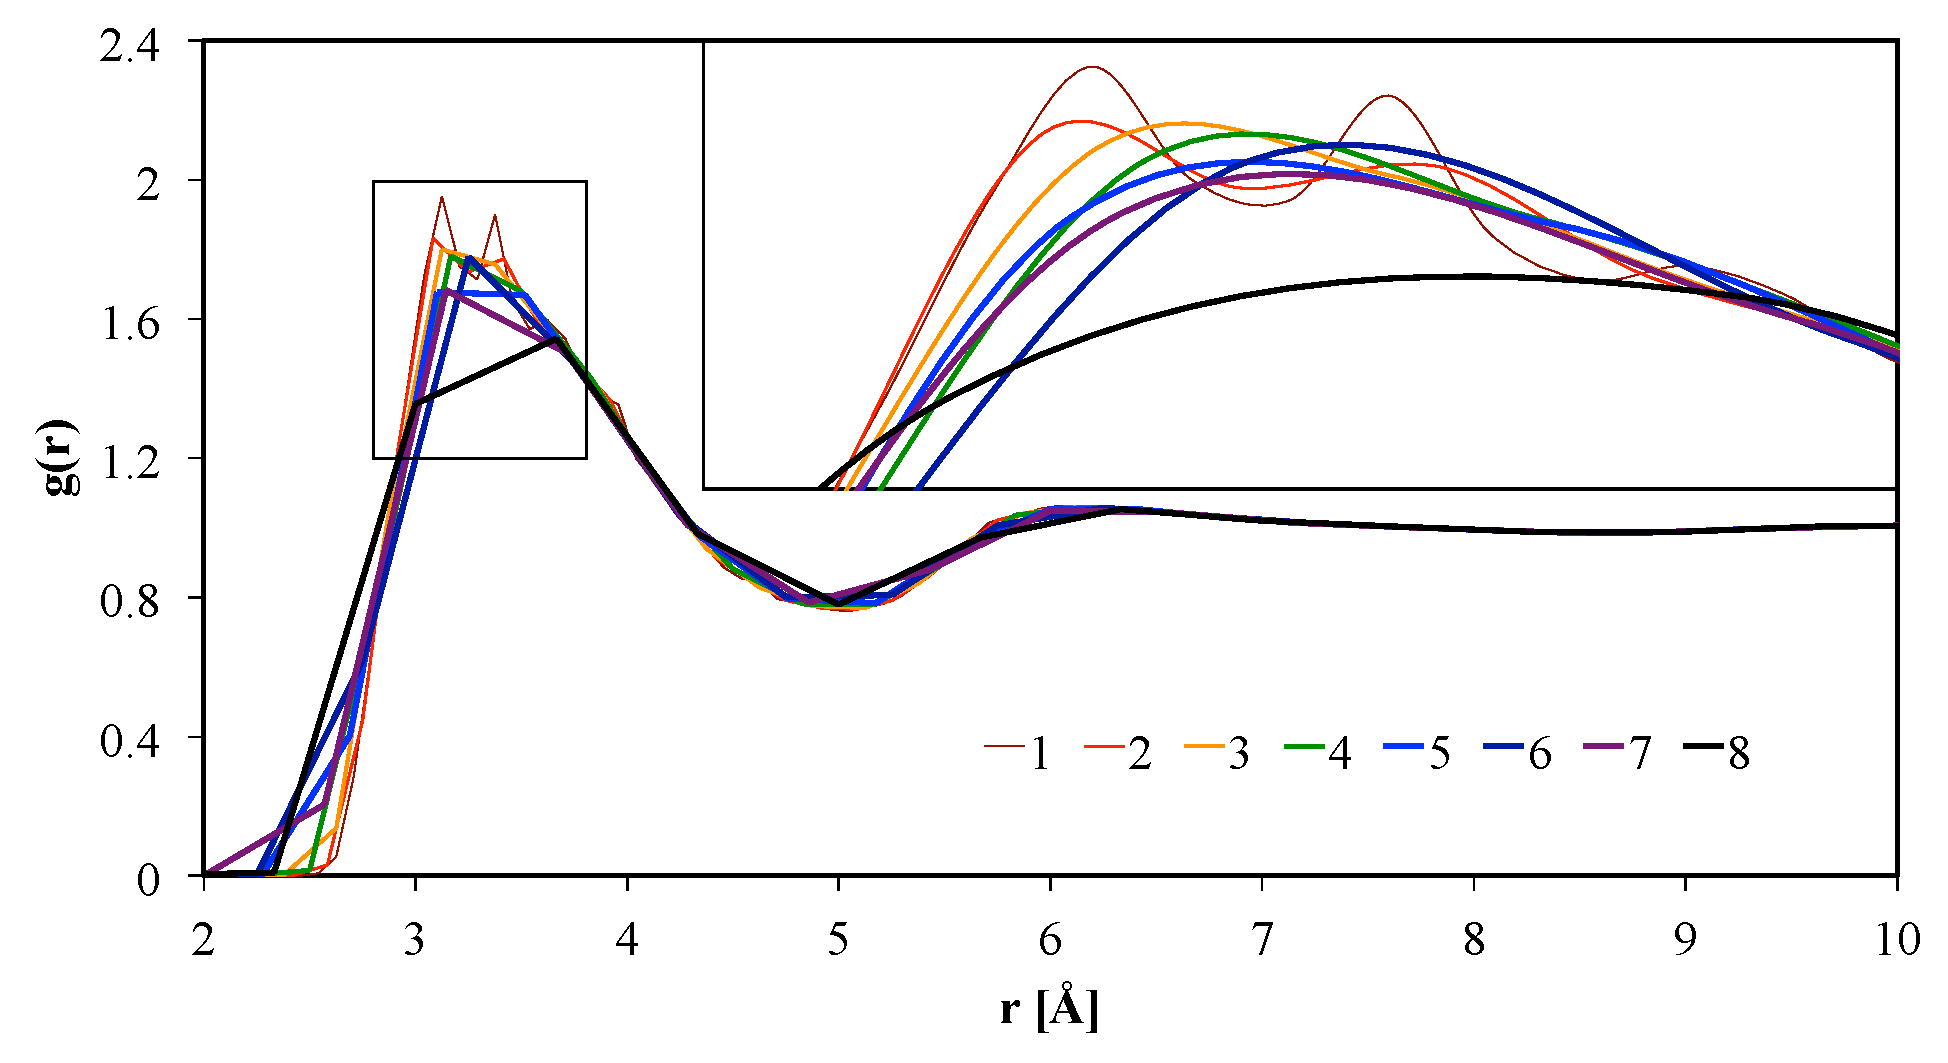
\includegraphics[bb=0cm 0.6cm 33cm 18cm,width=0.8\columnwidth]{_figure/results/rdf-smoothing}
\par\end{centering}
\caption[\acs{RDF} with different resolution parameter]{\acs{RDF} of site O in $\mathrm{O_{2}}$ molecule ($n_{\max}=4$,
$L=24$ $\textrm{Å}$, $\mathrm{nfft}=72$) with different resolution
parameter. The curves take $\frac{1}{N}n_{\mathrm{bin}}$ as number
of bins, with $n_{\mathrm{bin}}$ determined by the Rice rule, $N$
varying from 1 to 8. The square box on the left is zoomed and smoothed
(with Catmull-Rom spline implicitly used by Excel) in the right box.\label{fig:rdf-with-different}}
\end{figure}


\section{Generalized spherical harmonics transform\label{sec:gsh-imp}}

As discussed in $\mathsection$\ref{sec:fgsht}, a discretized function
$F(\Theta,\Phi,\Psi)$ after a forward-backward \acs{GSHT} process
(eq. (\ref{eq:GSHT-fwd}-\ref{eq:GSHT-bwd}))
\begin{equation}
F_{\mu'\mu}^{m}=\frac{f_{m}}{8\pi^{2}}\sum_{i=0}^{m_{\mathrm{max}}}w_{i}\sum_{j=0}^{2m_{\mathrm{max}}}\sum_{k=0}^{2\left\lfloor m_{\mathrm{max}}/s\right\rfloor }F(\Theta_{i},\Phi_{j},\Psi_{k})R_{\mu'\mu}^{m*}(\Theta_{i},\Phi_{j},\Psi_{k})\label{eq:f-ghst.1}
\end{equation}
\begin{equation}
F(\Theta_{i},\Phi_{j},\Psi_{k})=\sum_{m=0}^{n_{\mathrm{max}}}f_{m}\sum_{\mu'=-m}^{m}\sum_{\underset{\mod(\mu,s)=0}{\mu=-m}}^{m}F_{\mu'\mu}^{m}R_{\mu'\mu}^{m}(\Theta_{i},\Phi_{j},\Psi_{k})\label{eq:f-gsht.2}
\end{equation}
only remains the same when:
\begin{enumerate}
\item $F$ can be expanded on \acs{GSH}s of order at most $n_{\max}$ in
eq. (\ref{eq:f-gsht.2}), thus it is always the case that $F$ is
a polynomial of both $\cos\Theta$, $\cos\Phi$ and $\cos\Psi$ of
order $n$, where $n\leq n_{\max}$; 
\item The order of quadrature $m_{\max}$ used in the \acs{GSH} expansion
in eq. (\ref{eq:f-ghst.1}) should be larger than the order of the
polynomial $F$, which means $n\leq m_{\max}$;
\end{enumerate}
The two rules are quite evident. It should be also noted that as we
do first a forward then a backward transform, when $m_{\max}<n_{\max}$,
even the input function is of order at most $m_{\max}$; the output
function is of order $n_{\mathrm{max}}$ in the presence of $R_{\mu'\mu}^{m}$
which is of order $n_{\mathrm{max}}$. That means $F$ is no longer
the same. Therefore, the forward-backward error is also controlled
by the relation between the two discretizing parameters:
\begin{enumerate}
\item [3.]$m_{\max}\geq n_{\max}$ is needed to ensure the absence of accuracy
loss.
\end{enumerate}
In reality, the density variable $\rho(\mathbf{r},\mathbf{\Omega})$
and the gradient $\gamma(\mathbf{r},\mathbf{\Omega})$ that should
be expanded via \acs{FGSHT} are never a simple polynomial. It is
important to understand how much the choice of $m_{\max}$ and $n_{\max}$
will affect the accuracy, as they are tightly linked to the performance.
Therefore we chose some simple functions below to see what happens
when the function does not meet the three conditions. Note that the
\acs{FFT} process leads to strictly no accuracy loss (at machine
precision, approximatively $10^{-13}$), which means the \acs{FGSHT}
process will have strictly the same result with the \acs{GSHT} process.
Here we do not need to distinguish the two.

\subsection{$m_{\mathrm{max}}$ and $n_{\mathrm{max}}$ of projections}

The numerical error tests of a forward-backward \acs{GSHT} process
with different order $n_{\mathrm{max}}$ of \acs{GSH} and $m_{\mathrm{max}}$
of quadrature 
\begin{table}[!t]
\begin{centering}
\subfloat[$f(\mathbf{\Omega})=1$]{\begin{centering}
\begin{tabular*}{1\columnwidth}{@{\extracolsep{\fill}}ccccccc}
\toprule 
\addlinespace[-0.17em]
{\scriptsize{}$m$\textbackslash{}$n$} & {\scriptsize{}0} & {\scriptsize{}1} & {\scriptsize{}2} & {\scriptsize{}3} & {\scriptsize{}4} & {\scriptsize{}5}\tabularnewline
\midrule
\addlinespace[-0.33em]
{\scriptsize{}0} & \textbf{\scriptsize{}\uuline{0.00 (0.00)}} & {\scriptsize{}9.00 (3.00)} & {\scriptsize{}34.00 (18.00)} & {\scriptsize{}83.00 (39.00)} & {\scriptsize{}164.00 (84.00)} & {\scriptsize{}285.00 (139.00)}\tabularnewline
\addlinespace[-0.33em]
{\scriptsize{}1} & \textbf{\scriptsize{}\uuline{0.00 (0.00)}} & \textbf{\scriptsize{}\uuline{0.00 (0.00)}} & {\scriptsize{}0.00 (1.67)} & {\scriptsize{}4.34 (6.07)} & {\scriptsize{}7.06 (13.63)} & {\scriptsize{}14.88 (17.30)}\tabularnewline
\addlinespace[-0.33em]
{\scriptsize{}2} & \textbf{\scriptsize{}\uuline{0.00 (0.00)}} & \textbf{\scriptsize{}\uuline{0.00 (0.00)}} & \textbf{\scriptsize{}\uuline{0.00 (0.00)}} & {\scriptsize{}0.00 (0.00)} & {\scriptsize{}0.00 (0.00)} & {\scriptsize{}5.65 (2.71)}\tabularnewline
\addlinespace[-0.33em]
{\scriptsize{}3} & \textbf{\scriptsize{}\uuline{0.00 (0.00)}} & \textbf{\scriptsize{}\uuline{0.00 (0.00)}} & \textbf{\scriptsize{}\uuline{0.00 (0.00)}} & \textbf{\scriptsize{}\uuline{0.00 (0.00)}} & {\scriptsize{}0.00 (0.00)} & {\scriptsize{}0.00 (0.00)}\tabularnewline
\addlinespace[-0.33em]
{\scriptsize{}4} & \textbf{\scriptsize{}\uuline{0.00 (0.00)}} & \textbf{\scriptsize{}\uuline{0.00 (0.00)}} & \textbf{\scriptsize{}\uuline{0.00 (0.00)}} & \textbf{\scriptsize{}\uuline{0.00 (0.00)}} & \textbf{\scriptsize{}\uuline{0.00 (0.00)}} & {\scriptsize{}0.00 (0.00)}\tabularnewline
\addlinespace[-0.33em]
{\scriptsize{}5} & \textbf{\scriptsize{}\uuline{0.00 (0.00)}} & \textbf{\scriptsize{}\uuline{0.00 (0.00)}} & \textbf{\scriptsize{}\uuline{0.00 (0.00)}} & \textbf{\scriptsize{}\uuline{0.00 (0.00)}} & \textbf{\scriptsize{}\uuline{0.00 (0.00)}} & \textbf{\scriptsize{}\uuline{0.00 (0.00)}}\tabularnewline
\bottomrule
\end{tabular*}
\par\end{centering}
}
\par\end{centering}
\begin{centering}
\subfloat[$f(\mathbf{\Omega})=\cos3\Theta$]{\begin{centering}
\begin{tabular*}{1\columnwidth}{@{\extracolsep{\fill}}ccccccc}
\toprule 
\addlinespace[-0.17em]
{\scriptsize{}$m$\textbackslash{}$n$} & {\scriptsize{}0} & {\scriptsize{}1} & {\scriptsize{}2} & {\scriptsize{}3} & {\scriptsize{}4} & {\scriptsize{}5}\tabularnewline
\midrule
\addlinespace[-0.33em]
{\scriptsize{}0} & {\scriptsize{}0.00 (0.00)} & {\scriptsize{}0.00 (0.00)} & {\scriptsize{}0.00 (0.00)} & {\scriptsize{}0.00 (0.00)} & {\scriptsize{}0.00 (0.00)} & {\scriptsize{}0.00 (0.00)}\tabularnewline
\addlinespace[-0.33em]
{\scriptsize{}1} & {\scriptsize{}0.96 (0.96)} & {\scriptsize{}0.00 (0.00)} & {\scriptsize{}0.00 (0.00)} & {\scriptsize{}2.56 (6.99)} & {\scriptsize{}10.76 (14.15)} & {\scriptsize{}13.83 (21.21)}\tabularnewline
\addlinespace[-0.33em]
{\scriptsize{}2} & {\scriptsize{}0.46 (0.46)} & {\scriptsize{}0.00 (0.00)} & {\scriptsize{}0.00 (0.00)} & {\scriptsize{}0.00 (0.00)} & {\scriptsize{}0.00 (0.00)} & {\scriptsize{}1.36 (0.50)}\tabularnewline
\addlinespace[-0.33em]
{\scriptsize{}3} & {\scriptsize{}0.86 (0.86)} & {\scriptsize{}0.66 (0.66)} & {\scriptsize{}0.66 (0.66)} & \textbf{\scriptsize{}\uuline{0.00 (0.00)}} & {\scriptsize{}0.00 (0.00)} & {\scriptsize{}0.66 (0.66)}\tabularnewline
\addlinespace[-0.33em]
{\scriptsize{}4} & {\scriptsize{}0.99 (0.99)} & {\scriptsize{}0.80 (0.80)} & {\scriptsize{}0.80 (0.80)} & \textbf{\scriptsize{}\uuline{0.00 (0.00)}} & \textbf{\scriptsize{}\uuline{0.00 (0.00)}} & {\scriptsize{}0.00 (0.00)}\tabularnewline
\addlinespace[-0.33em]
{\scriptsize{}5} & {\scriptsize{}0.83 (0.83)} & {\scriptsize{}1.01 (1.01)} & {\scriptsize{}1.01 (1.01)} & \textbf{\scriptsize{}\uuline{0.00 (0.00)}} & \textbf{\scriptsize{}\uuline{0.00 (0.00)}} & \textbf{\scriptsize{}\uuline{0.00 (0.00)}}\tabularnewline
\bottomrule
\end{tabular*}
\par\end{centering}
}
\par\end{centering}
\begin{centering}
\subfloat[$f(\mathbf{\Omega})=\cos3\Phi$]{\begin{centering}
\begin{tabular*}{1\columnwidth}{@{\extracolsep{\fill}}ccccccc}
\toprule 
\addlinespace[-0.17em]
{\scriptsize{}$m$\textbackslash{}$n$} & {\scriptsize{}0} & {\scriptsize{}1} & {\scriptsize{}2} & {\scriptsize{}3} & {\scriptsize{}4} & {\scriptsize{}5}\tabularnewline
\midrule
\addlinespace[-0.33em]
{\scriptsize{}0} & {\scriptsize{}0.00 (0.00)} & {\scriptsize{}9.00 (3.00)} & {\scriptsize{}34.00 (18.00)} & {\scriptsize{}83.00 (39.00)} & {\scriptsize{}164.00 (84.00)} & {\scriptsize{}285.00 (139.00)}\tabularnewline
\addlinespace[-0.33em]
{\scriptsize{}1} & {\scriptsize{}0.00 (0.00)} & {\scriptsize{}0.00 (0.00)} & {\scriptsize{}0.00 (1.67)} & {\scriptsize{}4.34 (6.07)} & {\scriptsize{}7.06 (13.63)} & {\scriptsize{}14.88 (17.30)}\tabularnewline
\addlinespace[-0.33em]
{\scriptsize{}2} & {\scriptsize{}1.00 (1.00)} & {\scriptsize{}1.00 (1.00)} & {\scriptsize{}0.50 (0.50)} & {\scriptsize{}1.53 (1.53)} & {\scriptsize{}1.15 (1.15)} & {\scriptsize{}3.65 (0.89)}\tabularnewline
\addlinespace[-0.33em]
{\scriptsize{}3} & {\scriptsize{}1.00 (1.00)} & {\scriptsize{}1.00 (1.00)} & {\scriptsize{}1.00 (1.00)} & {\scriptsize{}0.83 (0.83)} & {\scriptsize{}1.10 (1.10)} & {\scriptsize{}1.11 (1.11)}\tabularnewline
\addlinespace[-0.33em]
{\scriptsize{}4} & {\scriptsize{}1.00 (1.00)} & {\scriptsize{}1.00 (1.00)} & {\scriptsize{}1.00 (1.00)} & {\scriptsize{}0.90 (0.90)} & {\scriptsize{}0.90 (0.90)} & {\scriptsize{}0.69 (0.69)}\tabularnewline
\addlinespace[-0.33em]
{\scriptsize{}5} & {\scriptsize{}1.00 (1.00)} & {\scriptsize{}1.00 (1.00)} & {\scriptsize{}1.00 (1.00)} & {\scriptsize{}0.94 (0.94)} & {\scriptsize{}0.94 (0.94)} & {\scriptsize{}0.80 (0.80)}\tabularnewline
\bottomrule
\end{tabular*}
\par\end{centering}
}
\par\end{centering}
\begin{centering}
\subfloat[$f(\mathbf{\Omega})=R_{30}^{3}(\mathbf{\Omega})$]{\begin{centering}
\begin{tabular*}{1\columnwidth}{@{\extracolsep{\fill}}ccccccc}
\toprule 
\addlinespace[-0.17em]
{\scriptsize{}$m$\textbackslash{}$n$} & {\scriptsize{}0} & {\scriptsize{}1} & {\scriptsize{}2} & {\scriptsize{}3} & {\scriptsize{}4} & {\scriptsize{}5}\tabularnewline
\midrule
\addlinespace[-0.33em]
{\scriptsize{}0} & {\scriptsize{}0.00 (0.00)} & {\scriptsize{}5.03 (1.68)} & {\scriptsize{}19.01 (10.06)} & {\scriptsize{}46.40 (21.80)} & {\scriptsize{}91.68 (46.96)} & {\scriptsize{}- (77.70)}\tabularnewline
\addlinespace[-0.33em]
{\scriptsize{}1} & {\scriptsize{}0.00 (0.00)} & {\scriptsize{}0.00 (0.00)} & {\scriptsize{}0.00 (0.51)} & {\scriptsize{}1.32 (1.85)} & {\scriptsize{}2.15 (4.15)} & {\scriptsize{}4.53 (5.26)}\tabularnewline
\addlinespace[-0.33em]
{\scriptsize{}2} & {\scriptsize{}0.56 (0.56)} & {\scriptsize{}0.56 (0.56)} & {\scriptsize{}0.07 (0.07)} & {\scriptsize{}0.55 (0.55)} & {\scriptsize{}0.76 (0.76)} & {\scriptsize{}2.05 (1.00)}\tabularnewline
\addlinespace[-0.33em]
{\scriptsize{}3} & {\scriptsize{}0.47 (0.47)} & {\scriptsize{}0.47 (0.47)} & {\scriptsize{}0.47 (0.47)} & \textbf{\scriptsize{}\uuline{0.00 (0.00)}} & {\scriptsize{}0.46 (0.46)} & {\scriptsize{}0.46 (0.46)}\tabularnewline
\addlinespace[-0.33em]
{\scriptsize{}4} & {\scriptsize{}0.56 (0.56)} & {\scriptsize{}0.56 (0.56)} & {\scriptsize{}0.56 (0.56)} & \textbf{\scriptsize{}\uuline{0.00 (0.00)}} & \textbf{\scriptsize{}\uuline{0.00 (0.00)}} & {\scriptsize{}0.00 (0.00)}\tabularnewline
\addlinespace[-0.33em]
{\scriptsize{}5} & {\scriptsize{}0.51 (0.51)} & {\scriptsize{}0.51 (0.51)} & {\scriptsize{}0.51 (0.51)} & \textbf{\scriptsize{}\uuline{0.00 (0.00)}} & \textbf{\scriptsize{}\uuline{0.00 (0.00)}} & \textbf{\scriptsize{}\uuline{0.00 (0.00)}}\tabularnewline
\bottomrule
\end{tabular*}
\par\end{centering}
}
\par\end{centering}
\caption[Maximum absolute error $E_{a}^{\mathrm{max}}$ of some function $f(\mathbf{\Omega})$
introduced by a forward-backward GSHT process]{Maximum absolute error $E_{a}^{\mathrm{max}}$ of some function $f(\mathbf{\Omega})$
introduced by a forward-backward \acs{GSHT} process, with $s=1$
outside the parentheses and $s=2$ inside the parentheses; $s$ being
the \acs{MRSO} defined in $\mathsection$\ref{sec:fgsht} concerning
the $\mathrm{C}_{2v}$ symmetry. Differences that should be theoretically
null (at machine precision) are shown in bold character and double
underlined; which are null in fact at machine precision and here presented
with 2 decimals for simpleness. \label{tab:error-gsh}}
\end{table}
are shown in table \ref{tab:error-gsh} for various polynomials; the
absolute error
\begin{equation}
E_{\mathrm{a}}(\mathbf{\Omega})=\left|f^{\mathrm{before}}(\mathbf{\Omega})-f^{\mathrm{after}}(\mathbf{\Omega})\right|
\end{equation}
being defined as the norm of difference in function $f(\mathbf{\Omega})$
after a forward-backward \acs{GSHT} process. The maximum absolute
error $E_{a}^{\mathrm{max}}$ is the maximum value in $E_{\mathrm{a}}(\mathbf{\Omega})$.

From table \ref{tab:error-gsh} we can see that for function $f(\mathbf{\Omega})=1=R_{00}^{0}$,
$m_{\max}\geq0$, $n_{\max}\geq0$ and $m_{\max}\geq n_{\max}$ give
a null difference. Similarly, function $f(\mathbf{\Omega})=\cos3\Theta=4\cos^{3}\Theta-3\cos\Theta$
is a polynomial of $\cos\Theta$ of order 3, which can be expanded
on $R_{00}^{3}$ and $R_{00}^{1}$ terms; it should satisfy $m_{\max}\geq n_{\max}\geq3$.
$f(\mathbf{\Omega})=\cos3\Phi$ is a polynomial of $\cos\Phi$ of
order 3, but it cannot be expanded on \acs{GSH}s. In fact, all the
functions in which the order of $\cos\Phi$ and $\cos\Psi$ is greater
than $\cos\Theta$ cannot be expanded on a finite number of \acs{GSH}s.
$R_{30}^{3}$ can be expanded on itself, and indeed a polynomial of
order 3 requiring $m_{\max}\geq n_{\max}\geq3$.

We can see that all the $E_{a}^{\mathrm{max}}$ where $m_{\max}<n_{\max}$
is are rather large, and fortunately we use only $m_{\max}\geq n_{\max}$
in \acs{FGSHT} for numerical reasons. Yet the $E_{a}^{\mathrm{max}}$
for $m_{\max}\geq n_{\max}$ may not be negligle either, knowing that
the values of trigonometric functions are between $\left[-1,1\right]$.
However, if the greatest portion of the function is a polynomial within
the required order, the extra part does not play a great role, and the
total mean error will not be as significant as seen now. 

\subsection{From $\rho$ to $\gamma$}

In the same way, the maximum absolute error of the density variable
$\rho(\mathbf{r},\mathbf{\Omega})$, which is not a combination of
\acs{GSH}s, can be huge. It even gives the appearance of unphysical
density $\rho(\mathbf{r},\mathbf{\Omega})<0$ (i.e. $\Delta\rho(\mathbf{r},\mathbf{\Omega})/\rho_{0}<-1$)
at certain points after a forward-backward \acs{GSHT} process, as
shown in figure \ref{fig:unphysical-rho}.

\begin{figure}[h]
\begin{centering}
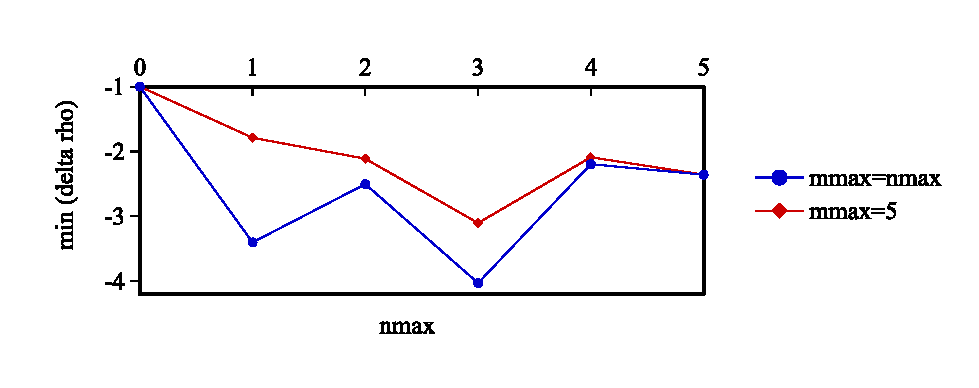
\includegraphics[bb=0bp 20bp 454bp 150bp,width=0.75\columnwidth]{_figure/results/min_delta_rho}
\par\end{centering}
\caption[The minimum value of $\Delta\rho(\mathbf{r},\mathbf{\Omega})/\rho_{0}$
after a forward-backward \acs{GSHT} process]{The minimum value of $\Delta\rho(\mathbf{r},\mathbf{\Omega})/\rho_{0}$
after a forward-backward \acs{GSHT} process with respect to $n_{\max}$.
Computed for a $45^{3}$ grid ($L=25$) for a converged density of
an artificial charged LJ center $\mathrm{CH}_{4}^{+0.4}$. \label{fig:unphysical-rho} }
\end{figure}

Theoretically, we expect this minimum value to approach zero when
increasing $m_{\max}$ or $n_{\max}$. This is not exactly the case.
That means the order of expansion within the computing capacity ($n_{\max}\leq5$)
is still far from finding a tendency. If we look at the rotational
invariant expansion of $\rho(\mathbf{r},\mathbf{\Omega})$, which
gives the projections $\rho_{0\nu}^{0nl}(r)$ \marginpar{It is normal that the curves in figure \ref{fig:rho.proj5Ind} and
\ref{fig:gamma.proj5Ind} are a little noised (with $n_{\mathrm{bin}}$)
as discussed above.}(0 as the solute is spherical) shown in figure \ref{fig:rho.proj5Ind},
\begin{figure}[h]
\begin{centering}
\subfloat[$\rho_{0\nu}^{0nl}(r)$ \label{fig:rho.proj5Ind}]{\begin{centering}
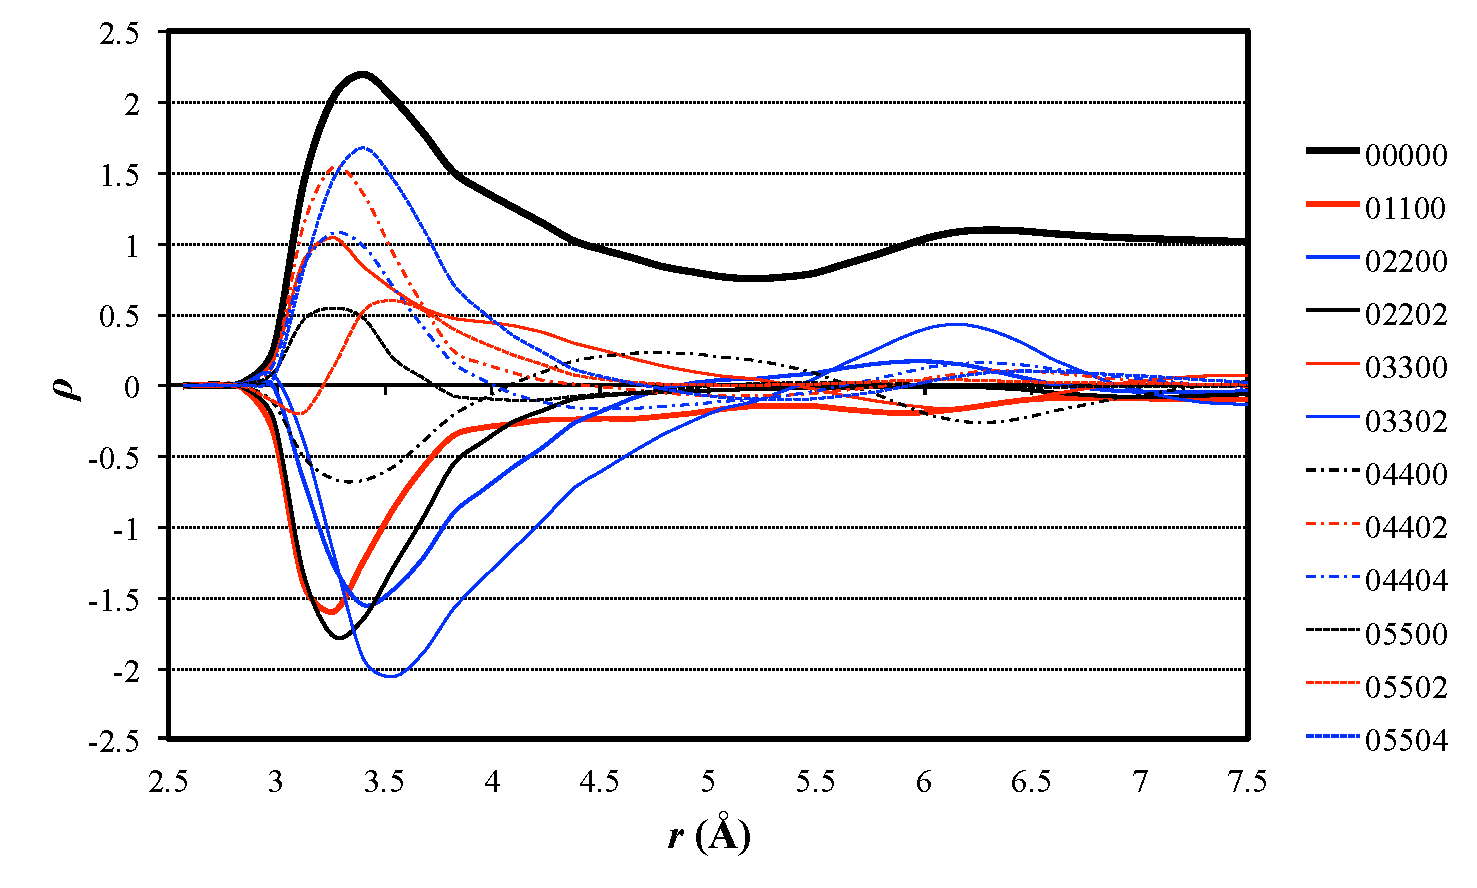
\includegraphics[bb=0cm 0.5cm 27cm 15cm,width=0.9\columnwidth]{_figure/results/rho}
\par\end{centering}
}
\par\end{centering}
\begin{centering}
\subfloat[$\gamma_{0\nu}^{0nl}(r)$\label{fig:gamma.proj5Ind}]{\begin{centering}
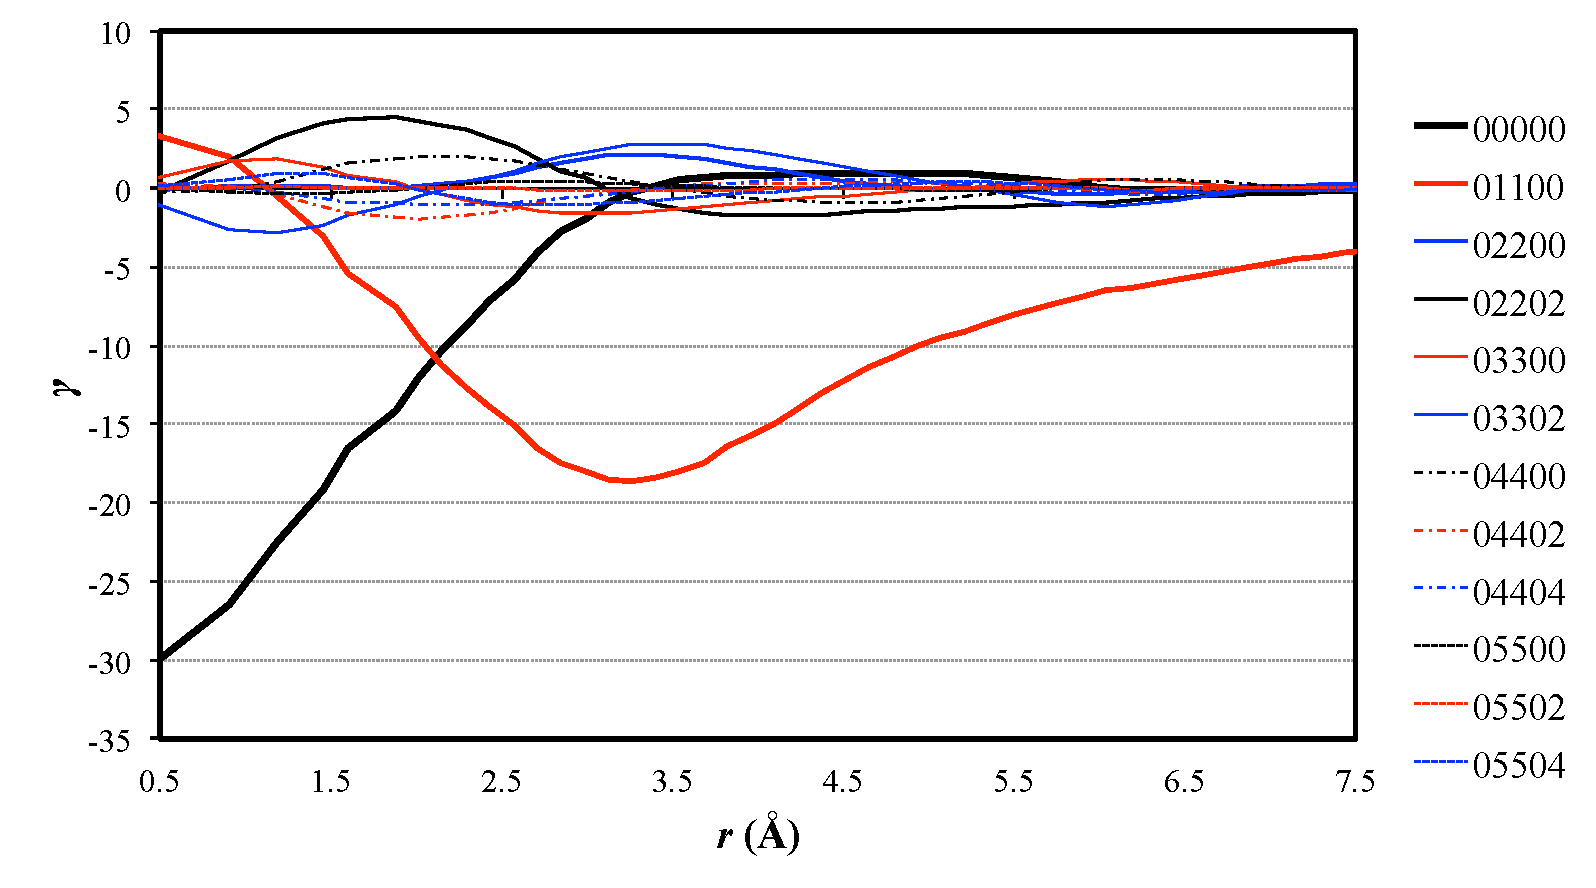
\includegraphics[bb=0cm 0.5cm 27cm 15cm,width=0.9\columnwidth]{_figure/results/gamma_convo}
\par\end{centering}
}
\par\end{centering}
\caption[$\rho_{0\nu}^{0nl}(r)$ and $\gamma_{0\nu}^{0nl}(r)$ of an artificial
charged LJ center $\mathrm{CH}_{4}^{+0.4}$]{The projections $\rho_{0\nu}^{0nl}(r)$ and $\gamma_{0\nu}^{0nl}(r)$
computed for a $45^{3}$ grid ($L=25$) for a converged density of
an artificial charged LJ center $\mathrm{CH}_{4}^{+0.4}$}
\end{figure}
we observe that the first peaks of higher order projections are still
non-negligible. That gives the tendency in figure \ref{fig:unphysical-rho}.
The first projection $\rho_{00}^{000}(r)$ is purely positive, such
that the minimum of $\rho$ is zero; when the more negative projections
are added on to the combined function, this error will go to negative.
The minimum will have a tendency to converge only if the order of
projections are above the current order 5.

That means within the computing capacity, we cannot correctly expand
the density $\rho$ on \acs{GSH}s. \marginpar{Note that the projections $f_{\mu\nu}^{mnl}$ are purely real if $f$
is real and $\mu$, $\nu$ are even numbers.}However, in the code MDFT, the density $\rho$ is generated by the
minimization process determined by the gradient of energy $\gamma$.
Note that $\hat{\gamma}(\mathbf{k},\mathbf{\Omega})$ is a convolution
product, where $\Delta\hat{\rho}(\mathbf{k},\mathbf{\Omega})$ and
the \acs{DCF} $\hat{c}(k,\mathbf{\Omega}_{1},\mathbf{\Omega}_{2})$
can be both expanded on \acs{GSH}s and rotational invariants. Therefore,
the higher order terms vanish more easily in $\hat{\gamma}$, as they
are the product of higher order terms of $\Delta\hat{\rho}(\mathbf{k},\mathbf{\Omega})$
and $\hat{c}(k,\mathbf{\Omega}_{1},\mathbf{\Omega}_{2})$. We see
in figure \ref{fig:gamma.proj5Ind} that the first terms of $\gamma$
are much stronger than the terms of $n=3,4,5$. Therefore we can consider
that the expansion of $\gamma$ already converges within $n_{\max}\leq5$,
even $n_{\max}\leq3$.

\section{Comparison between branches}

\begin{table}[!b]
\begin{centering}
\begin{tabular*}{1\linewidth}{@{\extracolsep{\fill}}lccc}
\toprule 
\addlinespace[-0.17em]
\tableheadline{{\footnotesize{}Method}} & {\scriptsize{}$n_{\max}$} & \tableheadline{{\footnotesize{}DCF}} & \tableheadline{{\footnotesize{}Free Energy}}{\scriptsize{} (kJ/mol)}\tabularnewline
\midrule
\addlinespace[-0.33em]
\texttt{\textbf{\scriptsize{}dipole}} & {\scriptsize{}1} & {\scriptsize{}\citep{zhao_accurate_2013}} & {\scriptsize{}13.965}\tabularnewline
\addlinespace[-0.33em]
\texttt{\textbf{\scriptsize{}naive\_dipole}} & {\scriptsize{}1} & {\scriptsize{}\citep{zhao_accurate_2013}} & {\scriptsize{}13.965}\tabularnewline
\addlinespace[-0.33em]
\texttt{\textbf{\scriptsize{}convolution\_standard}} & {\scriptsize{}1} & {\scriptsize{}\citep{zhao_accurate_2013}} & {\scriptsize{}13.965}\tabularnewline
\midrule 
\addlinespace[-0.33em]
\texttt{\textbf{\scriptsize{}naive\_standard}} & {\scriptsize{}1} & {\scriptsize{}\citep{puibasset_bridge_2012}} & {\scriptsize{}19.224}\tabularnewline
\addlinespace[-0.33em]
\texttt{\textbf{\scriptsize{}naive\_interpolation}} & {\scriptsize{}1} & {\scriptsize{}\citep{puibasset_bridge_2012}} & {\scriptsize{}19.434}\tabularnewline
\addlinespace[-0.33em]
\texttt{\textbf{\scriptsize{}naive\_nmax1}} & {\scriptsize{}1} & {\scriptsize{}\citep{puibasset_bridge_2012}} & {\scriptsize{}19.225}\tabularnewline
\addlinespace[-0.33em]
\texttt{\textbf{\scriptsize{}convolution\_standard}} & {\scriptsize{}1} & {\scriptsize{}\citep{puibasset_bridge_2012}} & {\scriptsize{}19.225}\tabularnewline
\addlinespace[-0.33em]
\texttt{\textbf{\scriptsize{}convolution\_asymm}} & {\scriptsize{}1} & {\scriptsize{}\citep{puibasset_bridge_2012}} & {\scriptsize{}19.225}\tabularnewline
\addlinespace[-0.33em]
\texttt{\textbf{\scriptsize{}convolution\_pure\_angular}} & {\scriptsize{}1} & {\scriptsize{}\citep{puibasset_bridge_2012}} & {\scriptsize{}19.225}\tabularnewline
\midrule 
\addlinespace[-0.33em]
\texttt{\textbf{\scriptsize{}naive\_standard}} & {\scriptsize{}3} & {\scriptsize{}\citep{puibasset_bridge_2012}} & {\scriptsize{}26.105}\tabularnewline
\addlinespace[-0.33em]
\texttt{\textbf{\scriptsize{}naive\_interpolation}} & {\scriptsize{}3} & {\scriptsize{}\citep{puibasset_bridge_2012}} & {\scriptsize{}26.971}\tabularnewline
\addlinespace[-0.33em]
\texttt{\textbf{\scriptsize{}convolution\_standard}} & {\scriptsize{}3} & {\scriptsize{}\citep{puibasset_bridge_2012}} & {\scriptsize{}26.105}\tabularnewline
\addlinespace[-0.33em]
\texttt{\textbf{\scriptsize{}convolution\_asymm}} & {\scriptsize{}3} & {\scriptsize{}\citep{puibasset_bridge_2012}} & {\scriptsize{}26.105}\tabularnewline
\addlinespace[-0.33em]
\texttt{\textbf{\scriptsize{}convolution\_pure\_angular}} & {\scriptsize{}3} & {\scriptsize{}\citep{puibasset_bridge_2012}} & {\scriptsize{}26.105}\tabularnewline
\bottomrule
\end{tabular*}
\par\end{centering}
\caption[Minimized free energy via different branches MDFT]{Minimized free energy via different branches MDFT of a charged $\mathrm{CH_{4}^{+0.33}}$
LJ center calculated for a $33^{3}$ ($L=20\textrm{Å}$) grid. Gauss-Legendre
quadrature is used as $\Theta$ angle grid, with $m_{\max}=n_{\max}$.\label{tab:free-energy}}
\end{table}
 

The algorithms mentioned in section \ref{chpt:algorithms-and-branches}
should give the same result if the same \acs{DCF} is used, on the
condition that the error due to discretization is not fatal. The most
direct comparison can be done with the free energy and structure obtained
at the end of minimization. To be more strict, it is also worthwhile
to study only the $\mathcal{F}_{\mathrm{exc}}$ functional evaluation
during one iteration without minimization, i.e. the process shown
in figure \ref{fig:Possible-algorithms}. In this scope, $\gamma(\mathbf{r},\mathbf{\Omega})$
becomes a better detailed criteria than $\mathcal{F}_{\mathrm{exc}}$
to be compared.

\subsection{Difference in energy evaluation}

Illustrated in table \ref{tab:free-energy}, the different methods
listed in table \ref{tab:Branch-option} and using the same \acs{DCF}
give nearly the same total free energy at the end of minimization.

In table \ref{tab:free-energy}, we can see that apart from \texttt{\textbf{naive\_interpolation}},
all branches give the same result if other parameters are fixed. The
slight difference due to the interpolation error is also acceptable
(in this case); and the error due to the \acs{GSH} expansion (difference
between, for instance, \texttt{\textbf{naive\_standard}} and \texttt{\textbf{convolution\_standard}})
seems to be well compensated during the minimization. This also supports
the conclusion above that in fact we just need a lower expansion of
\acs{GSH} for $\gamma$ than for $\Delta\rho$.

\subsection{A single $k$-kernel\label{subsec:A-single-k-kernel}}

If we want to compare within one evaluation of $\mathcal{F}_{\mathrm{exc}}$
as shown in figure \ref{fig:Possible-algorithms}, we can first
examine the local paths from $\Delta\hat{\rho}_{\mu'\mu}^{m}(\mathbf{k})$
to $\hat{\gamma}_{\mu'\mu}^{m}(\mathbf{k})$ that can be tested independently
for a given $\mathbf{k}$. Referring to figure \ref{fig:k-kernel},
four algorithms are available for such a purpose:

\begin{figure}[h]
\begin{centering}
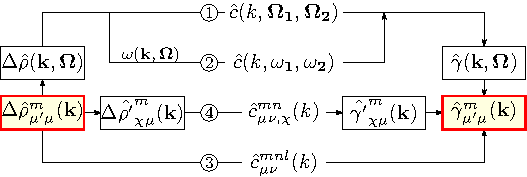
\includegraphics{_figure/algorithms_q}
\par\end{centering}
\caption{A $k$-kernel\label{fig:k-kernel}}
\end{figure}

A program to compare each element of $\hat{\gamma}_{\mu'\mu}^{m}(\mathbf{k})$
issued from these four algorithms for a given $\Delta\hat{\rho}_{\mu'\mu}^{m}(\mathbf{k})$
shows that the $\hat{\gamma}_{\mu'\mu}^{m}(\mathbf{k})$ for the four
algorithms are strictly identical, i.e. the maximum error is at machine
precision. This means the final result of energy and structure is
independent to the choice of path inside a $k$-kernel, if $\Delta\hat{\rho}(\mathbf{k},\mathbf{\Omega})$
can be fully expanded on \acs{GSH}s.

\subsection{$k$-border effect\label{subsec:k-border-effect}}

The next step is to test the whole process shown in figure \ref{fig:Possible-algorithms}.
Theoretically, if $\Delta\rho(\mathbf{r},\mathbf{\Omega})$ is generated
from a recombination of \acs{GSH} projections $\Delta\rho_{\mu'\mu}^{m}(\mathbf{r})$,
all the branches should give mathematically the same gradient $\gamma(\mathbf{r},\mathbf{\Omega})$. 

\marginpar{The detailed error value of $\gamma$ here has not been noted, as
it was regarded as a bug in the code at that time, but the code has
since been modified. In fact, the choice to add corrections or
not on the even number grid is not a matter of right and wrong.}Firstly, we compare the three \texttt{\textbf{convolution}} algorithms
passing by \acs{GSH} expansion. For a $64^{3}$ grid, $n_{\max}=3$,
the three algorithms \texttt{\textbf{convolution\_standard}}, \texttt{\textbf{convolution\_asymm}},
and \texttt{\textbf{convolution\_pure\_angular}} give the same $\mathcal{F}_{\mathrm{exc}}$
at first sight, but somewhat different results when comparing each
element of $\gamma(\mathbf{r},\mathbf{\Omega})$. The perceived difference
seems to decrease when increasing the number of grid points. Moreover,
$\gamma(\mathbf{r},\mathbf{\Omega})$ recombined from projections
$\gamma_{\mu'\mu}^{m}(\mathbf{r})$, which should be purely real as
explained in $\mathsection$\ref{subsec:Reduction-by-symmetry}, have
a slight imaginary part. Surprisingly, for a $65^{3}$ grid, it gives
numerically the same $\gamma(\mathbf{r},\mathbf{\Omega})$ for all
three algorithms at machine precision. The theory behind this behavior
is found to be a special $k$-border effect linking to an even number
of nodes in any dimension of the grid.

As the symmetry
\begin{equation}
\Delta\hat{\rho'}_{\chi\mu}^{m}(\mathbf{k})=(-)^{m+\mu+\chi}\Delta\hat{\rho'}_{\chi\underline{\mu}}^{m*}(-\mathbf{k})\label{eq:2-1}
\end{equation}
 is generated by two symmetries
\begin{equation}
\Delta\hat{\rho}_{\mu'\mu}^{m}(\mathbf{k})=(-)^{\mu'+\mu}\Delta\hat{\rho}_{\underline{\mu'}\underline{\mu}}^{m*}(-\mathbf{k})\label{eq:1-1}
\end{equation}
\begin{equation}
R_{\mu'\chi}^{m}(\mathbf{\hat{k}})=(-)^{m+\mu'+\chi}R_{\underline{\mu'}\chi}^{m}(-\hat{\mathbf{k}})\label{eq:3-1}
\end{equation}

For the $k$ points ``at border'', i.e. after the \acs{FFT} where
the point having $\pm k_{i}=k_{i}^{\mathrm{max}}$, $i=1,2,3$, for
example for $k_{1}$,
\begin{equation}
\Delta\hat{\rho}_{\mu'\mu}^{m}(\pm k_{1},k_{2},k_{3})=\Delta\hat{\rho}_{\mu'\mu}^{m}(k_{1}^{\mathrm{max}},k_{2},k_{3})
\end{equation}
is naturally put in the same array by FFT for the grids of an even
number, as shown in figure \ref{fig:k-border-effect}. 

\begin{figure}[H]
\begin{centering}
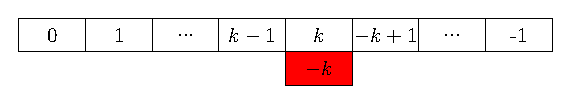
\includegraphics{_figure/k-border}
\par\end{centering}
\caption{$k$-border effect\label{fig:k-border-effect}}
\end{figure}
\marginpar{For example, for a grid 1D, the FFT having 6 points gives the values
for indices 0,1,2,3,-2,-1, and the FFT having 7 points gives the values
for 0,1,2,3,-3,-2,-1.}

As \acs{FFT} possesses periodicity, the symmetry (\ref{eq:1-1})
can always be respected at the border. However, as
\begin{equation}
R_{\underline{\mu'}\chi}^{m}(-\hat{k}\equiv(-k_{1},-k_{2},-k_{3}))\neq R_{\mu'\chi}^{m}(k_{1}^{\mathrm{max}},-k_{2},-k_{3})
\end{equation}
the symmetries (\ref{eq:3-1}) and (\ref{eq:2-1}) are not respected
for these points. In the backward process, if we account for all the
$\gamma_{\mu'\mu}^{m}(\mathbf{k})$, as
\begin{equation}
\gamma_{\mu'\mu}^{m}(-\hat{k}\equiv(-k_{1},-k_{2},-k_{3}))\neq\gamma_{\mu'\mu}^{m}(k_{1}^{\mathrm{max}},-k_{2},-k_{3})
\end{equation}
the symmetry
\begin{equation}
\gamma_{\mu'\mu}^{m}(\mathbf{k})=(-)^{\mu'+\mu}\gamma_{\underline{\mu'}\underline{\mu}}^{m*}(-\mathbf{k})\label{eq:4-1}
\end{equation}
is not totally respected, and this imposes that $\gamma_{\mu'\mu}^{m}(\mathbf{r})$
has a imaginary part. This imaginary part has been omitted implicitly
in the ``real to complex'' \acs{FFT} process used in, for example,
\acs{FGSHT} in \texttt{\textbf{convolution\_standard}}, or \acs{FFT}3D
in \texttt{\textbf{convolution\_pure\_angular}}. That is to say, we
keep only the part of nonnegative $\mathbf{k}$ or nonnegative $\mu$,
supposing that the part we omit respects the symmetry.

In the purpose that the three algorithm gives the same result, we
can artificially impose at the border:
\begin{equation}
R_{\mu'\chi}^{m}(k_{i}^{\mathrm{max}})=\frac{1}{2}\left[R_{\mu'\chi}^{m}(k_{i})+R_{\mu'\chi}^{m}(-k_{i})\right]
\end{equation}
where $i$ is the conflict index in figure \ref{fig:k-border-effect}.
If more than one dimension is in conflict, this process can be done
twice (4 terms for ``edges'' of the cube) or three times (8 terms
for ``vertices''). The point $\mathbf{k}=\hat{0}$ is different;
as it is defined along the $z$-axes to avoid underdetermination,
it does not respect eq. (\ref{eq:3-1}) and (\ref{eq:2-1}), neither.
However, this point is proven to be negligible compared to the hundreds
of thousands of total points.

\subsection{Difference in $\gamma$ for ``naive'' and ``convolution'' methods}

In the same way, we compare the $\mathcal{F}_{\mathrm{exc}}$ and
$\gamma(\mathbf{r},\mathbf{\Omega})$ given by branches \texttt{\textbf{naive\_standard}}
and \texttt{\textbf{convolution\_standard}}. The $\mathcal{F}_{\mathrm{exc}}$
of these two branches are identical for a $65^{3}$ and $n_{\max}=3$
grid, but the elements of $\gamma(\mathbf{r},\mathbf{\Omega})$ have
a difference at order of $10^{-2}$ to $10^{-3}$ which seems to be
random. A test redone for a $45^{3}$ grid is shown in figure \ref{fig:Difference-in-gamma}.

According to figure \ref{fig:Difference-in-gamma}, we can hypothesize
that this error depends on the angular quadrature $m_{\max}$. The
dependence is natural, as the difference between algorithms \texttt{\textbf{naive}}
and \texttt{\textbf{convolution}} is the treatment of the angular
part. There is also a dependence on $L$ in the $k$-space, but after
\acs{FFT} it is mixed. The increase of error in the $n_{\max}$ chart
is unnatural, implying there is still something theoretical that we
have missed, or a bug in the code.

In short, this troublesome difference cannot be yet explained, as
the \texttt{\textbf{naive}} methods do not have a $k$-border effect
linked to symmetry, and in fact we used an odd grid. The projections
$\gamma_{\mu\nu}^{mnl}(r)$ of these two algorithms seem to be identical
(figure \ref{fig:gamma-proj}), which is to say that the global profile
of the two should be almost the same, and thus the error would not
be very decisive. Knowing that the difference is even more compensated
with many iterations as shown in table \ref{tab:free-energy}, we
can consider that this slight difference has no consequence to the
final result.

\begin{figure}[!th]
\begin{centering}
\subfloat[{$\delta\left[k_{\mathrm{B}}T\rho_{0}\hat{\gamma}(\mathbf{k},\mathbf{\Omega})\right]$}]{\begin{centering}
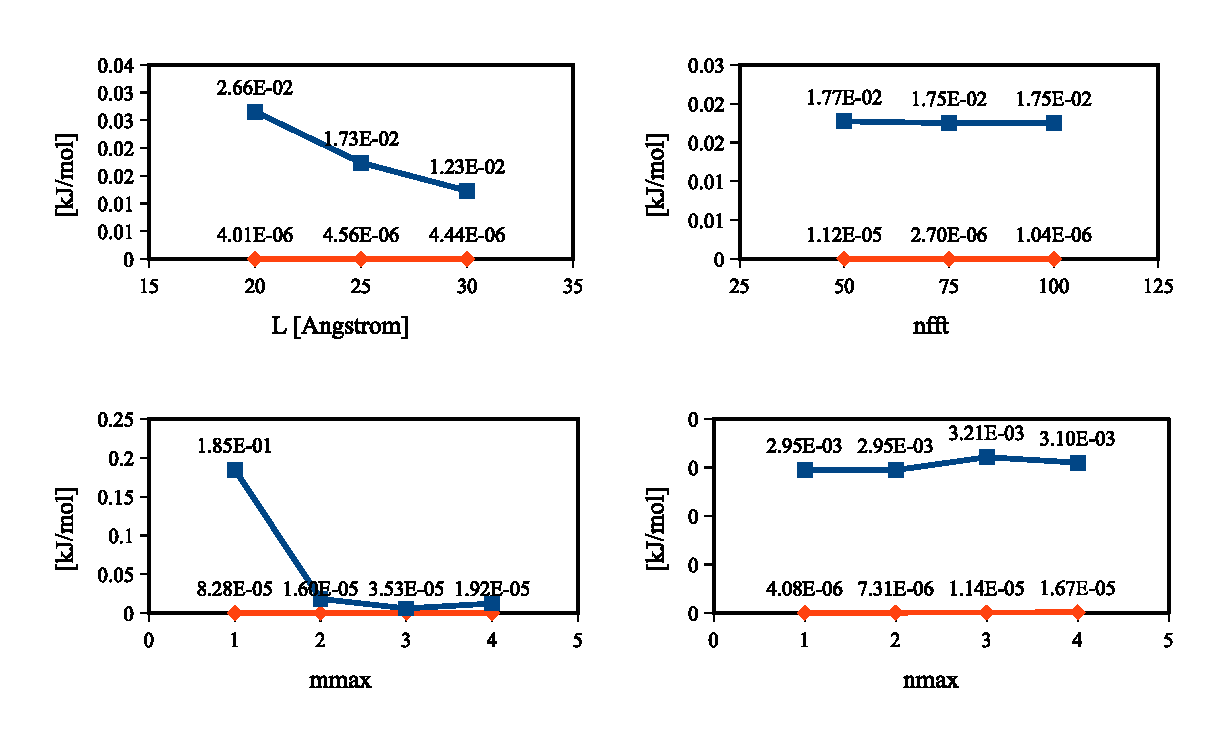
\includegraphics[bb=0bp 20bp 567bp 320bp,width=0.9\columnwidth]{_figure/results/diff_k_gamma}
\par\end{centering}
}
\par\end{centering}
\begin{centering}
\subfloat[{$\delta\left[k_{\mathrm{B}}T\rho_{0}\gamma(\mathbf{r},\mathbf{\Omega})\right]$}]{\begin{centering}
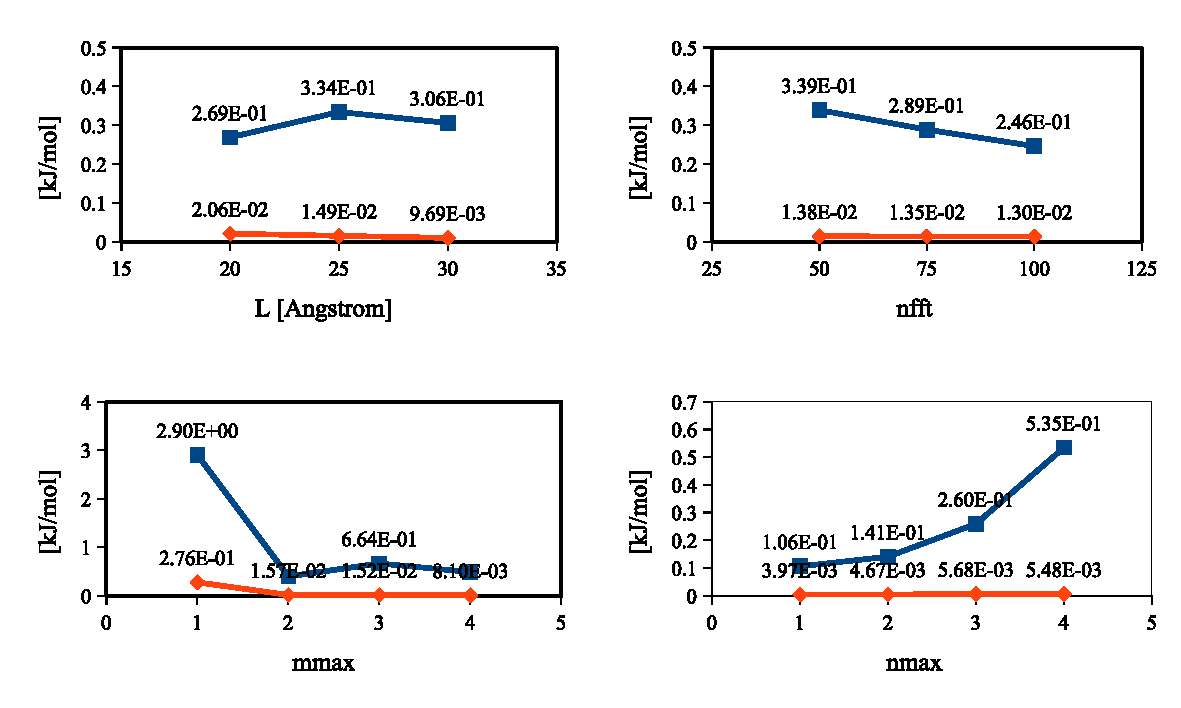
\includegraphics[bb=0bp 20bp 567bp 320bp,width=0.9\columnwidth]{_figure/results/diff_gamma}
\par\end{centering}
}
\par\end{centering}
\caption[Absolute differences in $\hat{\gamma}(\mathbf{k},\mathbf{\Omega})$
and $\gamma(\mathbf{r},\mathbf{\Omega})$]{Maximum (blue) and average (red) absolute difference in $\hat{\gamma}(\mathbf{k},\mathbf{\Omega})$
and $\gamma(\mathbf{r},\mathbf{\Omega})$ (normalized with $k_{\mathrm{B}}T\rho_{0}$),
for tests of: (1) different box length $L$, with $\mathrm{nfft}=65$,
$m_{\max}=n_{\max}=2$; (2) different number of grid $\mathrm{nfft}^{3}$,
with $L=25$ $\textrm{Å}$, $m_{\max}=n_{\max}=2$; (3) $n_{\max}=1$
to 4 for $m_{\max}=n_{\max}$ with $45^{3}$ grid ($L=25$ $\textrm{Å}$);
(4) $n_{\max}=1$ to 4 for $m_{\max}=5$ with $45^{3}$ grid ($L=25$
$\textrm{Å}$). The test of $m_{\max}=n_{\max}=5$ with $45^{3}$
grid ($L=25$ $\textrm{Å}$) is dropped as it takes too long. All
the tests uses a converged density $\rho(\mathbf{r},\mathbf{\Omega})$
of an artificial charged LJ center $\mathrm{CH}_{4}^{+0.4}$, recombined
from \acs{GSH} projections of corresponding order $m_{\max}$ and
$n_{\max}$. \label{fig:Difference-in-gamma}}
\end{figure}


\section{Intrinsic variation of free energy\label{sec:Intrinsic-variation-of}}

The comparison between branches shows that there is no significant
difference between the branches, if other parameters are all fixed.
Therefore we are free to study the dependence on discretizing parameters
with one or another algorithm. 

Before studying the dependence on expansion order $m_{\max}$ and
$n_{\max}$, we are interested in the spatial grid dependance, as
well as the $\Psi$ grid dependance if it is not automatically fixed
by $m_{\max}$ (figure \ref{fig:Space-grid-and-psi-dependence}),
which can have an influence on the tests later.

\begin{figure}[!tbph]
\begin{centering}
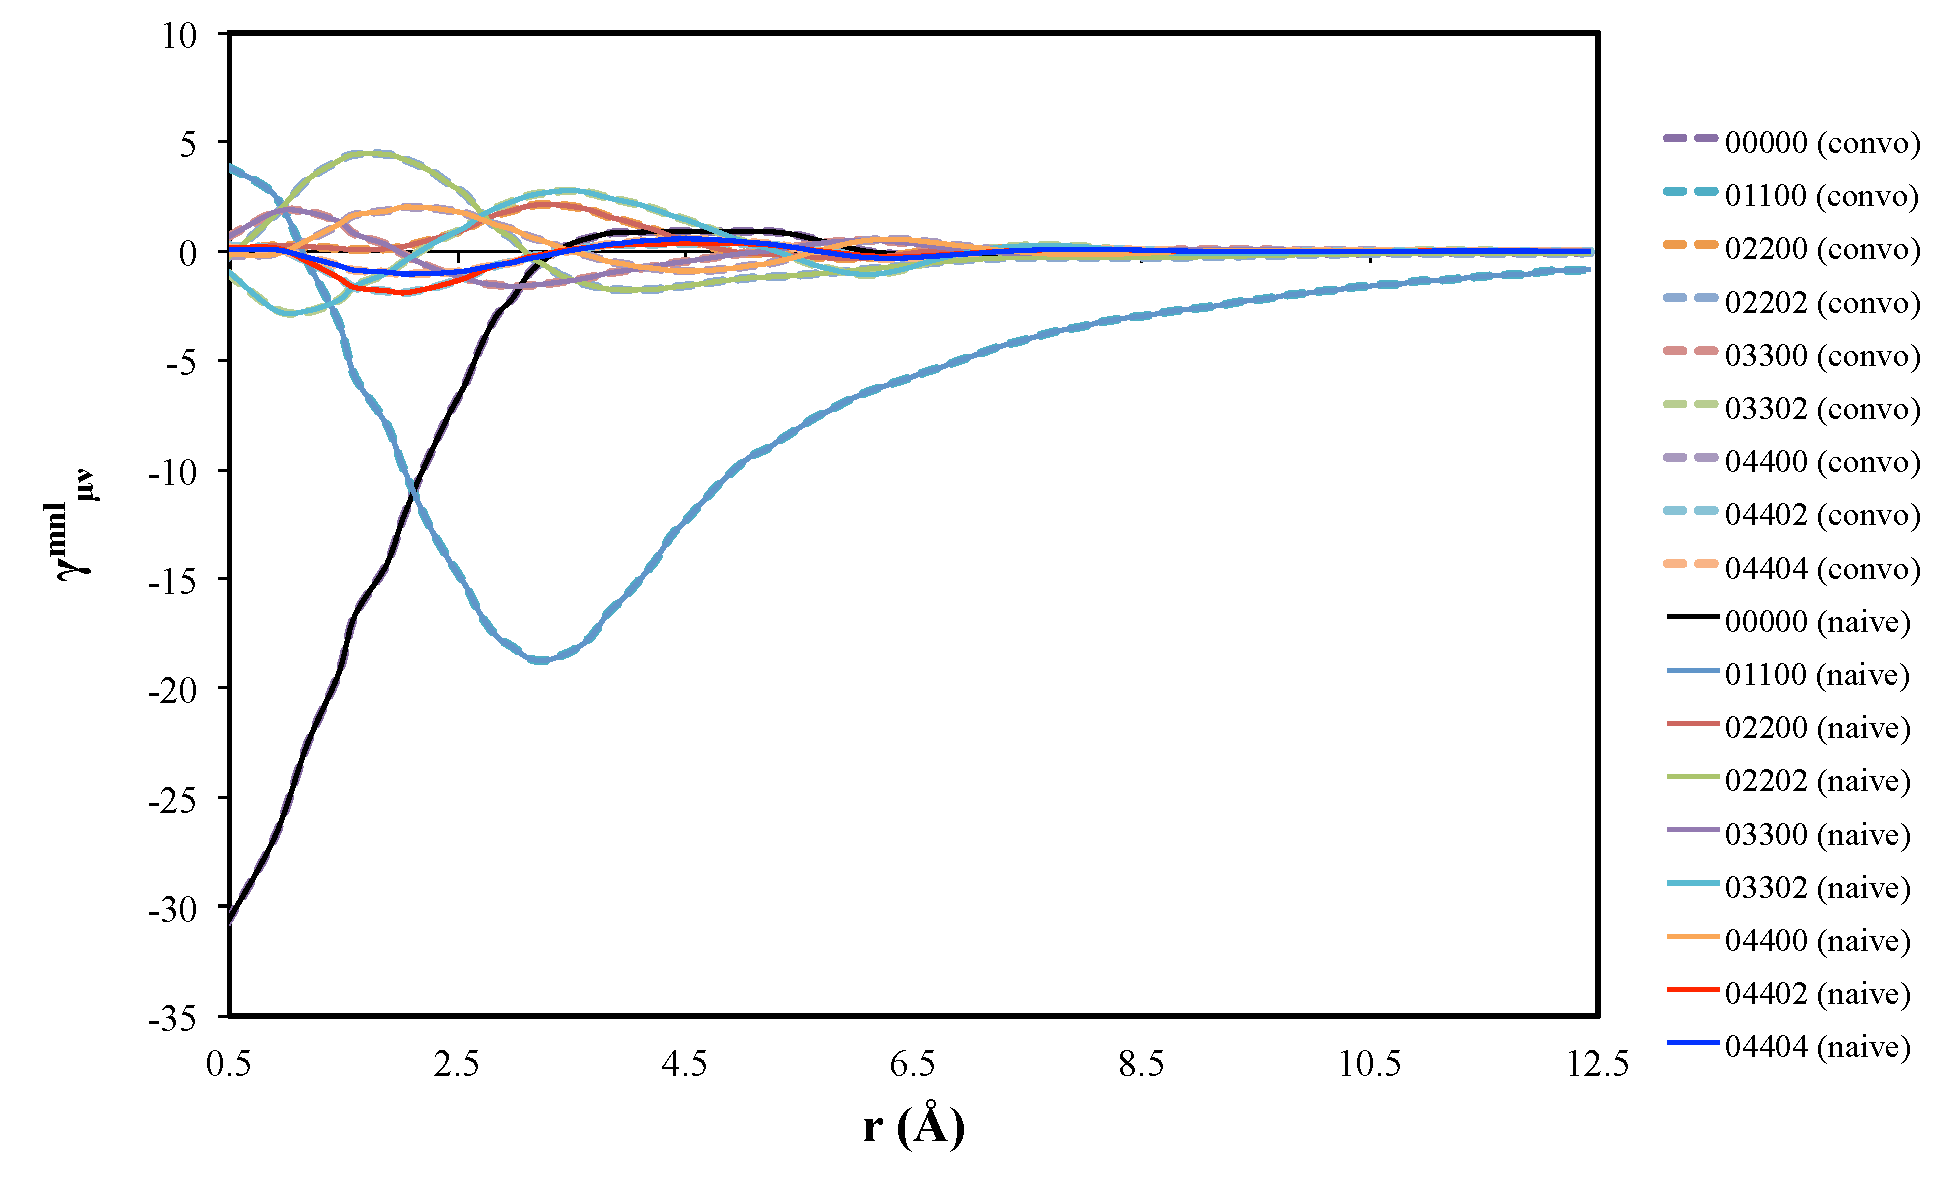
\includegraphics[width=0.85\columnwidth]{_figure/results/gamma_proj}
\par\end{centering}
\caption[Comparison of projections $\gamma_{0\nu}^{0nl}(r)$ for branches ``naive\_standard''
and ``convolution\_standard'']{Comparison of projections $\gamma_{0\nu}^{0nl}(r)$ for branches
``naive\_standard'' and ``convolution\_standard'', computed with
a $45^{3}$ grid ($L=25$) for a converged density of an artificial
charged LJ center $\mathrm{CH}_{4}^{+0.4}$.\label{fig:gamma-proj}}

\vspace{0.33cm}

\begin{centering}
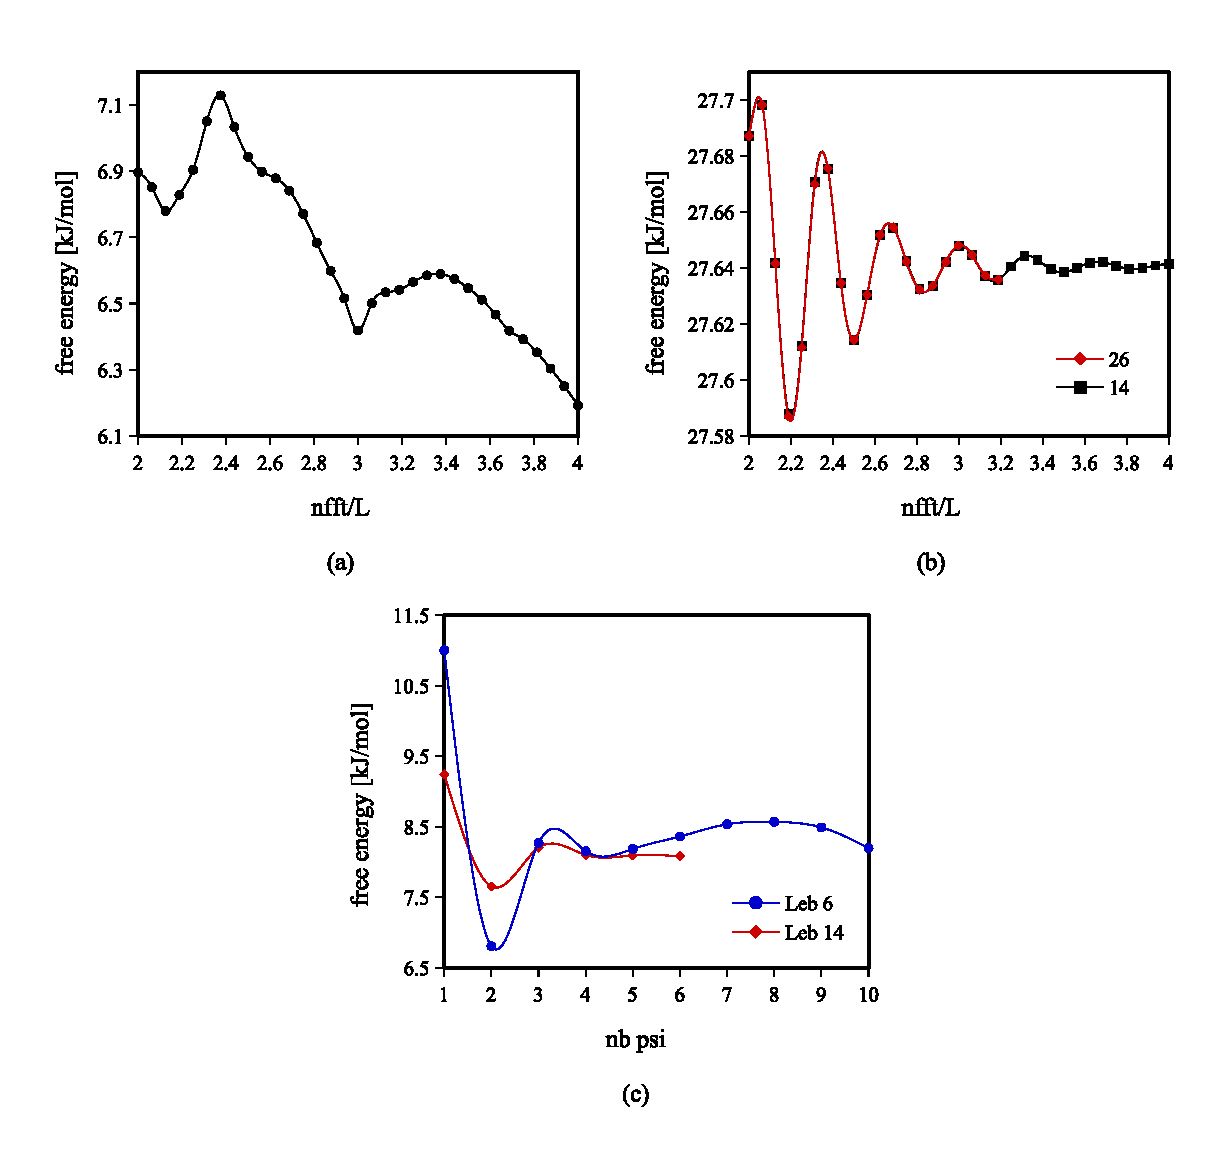
\includegraphics[bb=0bp 20bp 567bp 519bp,width=0.9\columnwidth]{_figure/results/grid_reso}
\par\end{centering}
\caption[Space-grid and $\Psi$ dependence of code MDFT]{Space-grid and $\Psi$ dependence of code \acs{MDFT}. (a) $\mathrm{CH_{4}^{+0.33}}$
using dipole \acs{DCF} with $n_{\max}=1$, $L=32$ $\textrm{Å}$;
(b) $\mathrm{CH_{4}}$ using \acs{DCF} of $n_{\max}=5$, $L=32$
$\textrm{Å}$, Lebedev quadrature of order 2 or 3; (c) acetone using
dipole \acs{DCF}, Lebedev quadrature 1 and 1$\Psi$ angles, $\mathrm{nfft}/L=2,3,4$,
using direct summation; (d) acetone using dipole \acs{DCF} and Lebedev
quadrature 1 or 2, varying $\Psi$, $L=32$ $\textrm{Å}$, $\mathrm{nfft}=96$.\label{fig:Space-grid-and-psi-dependence}}
\end{figure}

Looking at figure \ref{fig:Space-grid-and-psi-dependence} (a) and
(b), we show that the resolution of the spatial grid has an effect
on the calculated free energy. For the charged solute $\mathrm{CH_{4}^{+0.33}}$,
the energy has a tendency to decrease when increasing the resolution
of grid (nfft). This decrease does not link to the border correction
mentioned in $\mathsection$\ref{sec:Free-energy-correction}, as
both the box length and the charge remain the same for the whole set
of test. From (b) we consider that at least a 3 points grid in 1 dimension
(each direction) per Angstrom is needed to reduce the uncertainty
due to grid resolution. The molecule in Figure (c) is neutral (although
dipolar), i.e. does not need any border correction neither. We see
that the energy also varies with respect to the box length (with direct
summation this time), and have the same tendency for different resolution
$\mathrm{nfft}/L$. The curves of $\mathrm{nfft}/L=3$ and $\mathrm{nfft}/L=4$
do not give too much difference. Figure (d) fixed the Lebedev quadrature
for $\Theta$ and $\Phi$, but left varying the $\Psi$. We can also
see a dependence on $\Psi$ which does not completely vanish when
increasing the resolution of angular grid. Since during the whole
thesis the $\Psi$ is theoretically fixed by the order of the quadrature
in $\Theta$ and $\Phi$, this remains an issue for further verification.
We can roughly conclude that an error around 1-2 kJ/mol is common
for this code. The spatial grid dependence will not be treated in
this thesis as it may come from other terms of the functional.

\section{Series of charged LJ centers}

To validate the method by comparing with \acs{IET}, as well as to
study the dependance on $m_{\max}$ and $n_{\max}$, we firstly chose
a series of charged LJ centers, which possess the LJ parameters of
$\mathrm{C}\mathrm{H}_{4}$ \citep{asthagiri_role_2008}, and have
a variable charge from -1.0 to 1.0 (table \ref{tab:Parameters-of-charged-met}).\marginpar{For both IET and DM results in this thesis, 298K is used according
to habitude instead of 303K recommended in reference \citep{SPC/E}.
For MDFT, 300K and 298K are used.}

\begin{table}[h]
\begin{centering}
\begin{tabular*}{1\linewidth}{@{\extracolsep{\fill}}cccc}
\toprule 
\tableheadline{Solute} & $\mathfrak{q}$ & $\sigma$ {[}$\textrm{Å}${]} & $\epsilon$ {[}$\mathrm{kJ\cdot mol^{-1}}${]}\tabularnewline
\midrule
$\mathrm{C}\mathrm{H}_{4}$  & -1.0 to 1.0 & 3.73  & 1.23 \tabularnewline
\bottomrule
\end{tabular*}
\par\end{centering}
\caption{Parameters of charged $\mathrm{C}\mathrm{H}_{4}$ LJ centers for test
usage\label{tab:Parameters-of-charged-met}}
\end{table}


\subsection{Box length dependance and charge dependance of free energy}

As discussed in section \ref{sec:Free-energy-correction}, for single
ions, two types of corrections need to be added on the free energy,
which depend on the box length and charge of the ion. To verify these
dependencies, we implement a systematic calculation with variable
charge and box length using 3 different methods, the parameters of
which are shown in table \ref{tab:parameters-ch4}. It should be noted
that, the \texttt{\textbf{naive\_interpolation}} only used 14 Lebedev
and 3 $\Psi$ angles to converge, which gives exactly the same result
with 26 Lebedev and 4 $\Psi$ angles. That means the \texttt{\textbf{naive}}
methods do not need an order of quadrature $m_{\max}$ to be greater
than the order of \acs{DCF} $n_{\max}$. \marginpar{Some points of negative charge diverged; (in \acs{IET}, the negative
charge also have difficulty to converge), and all the converged results
are presented.}

\begin{table}[h]
\begin{centering}
\begin{tabular*}{1\linewidth}{@{\extracolsep{\fill}}cccccc}
\toprule 
\addlinespace[-0.17em]
\tableheadline{{\footnotesize{}Method}} & \tableheadline{{\footnotesize{}Surname}} & {\scriptsize{}$L$} & {\scriptsize{}nfft/$L$} & {\scriptsize{}$m_{\max}$} & {\scriptsize{}$n_{\max}$}\tabularnewline
\midrule
\addlinespace[-0.33em]
\texttt{\textbf{\scriptsize{}naive\_nmax1}} & {\scriptsize{}nmax1\_lmn} & {\scriptsize{}24 to 60} & {\scriptsize{}3} & {\scriptsize{}1 (Leb), 3 angles for $\Psi$} & {\scriptsize{}1}\tabularnewline
\addlinespace[-0.33em]
\texttt{\textbf{\scriptsize{}naive\_interpolation}} & {\scriptsize{}nmax5\_inter} & {\scriptsize{}24 to 60} & {\scriptsize{}3} & {\scriptsize{}2 (Leb), 3 angles for $\Psi$} & {\scriptsize{}5}\tabularnewline
\addlinespace[-0.33em]
\texttt{\textbf{\scriptsize{}convolution\_standard}} & {\scriptsize{}nmax1\_convo} & {\scriptsize{}24 to 60} & {\scriptsize{}3} & {\scriptsize{}1} & {\scriptsize{}1}\tabularnewline
\bottomrule
\end{tabular*}
\par\end{centering}
\caption[Methods and parameters for charged $\mathrm{C}\mathrm{H}_{4}$ series
test]{Methods and parameters for charged $\mathrm{C}\mathrm{H}_{4}$ series
test. Leb is Lebedev quadrature (6 angles of $\Theta$ and $\Phi$
for $m_{\max}=1$ and 14 for $m_{\max}=2$), which is mathematically
equivalent to Gauss-Legendre quadrature but requires only ˜2/3 angles.\label{tab:parameters-ch4}}
\end{table}

\begin{figure}[!bh]
\begin{centering}
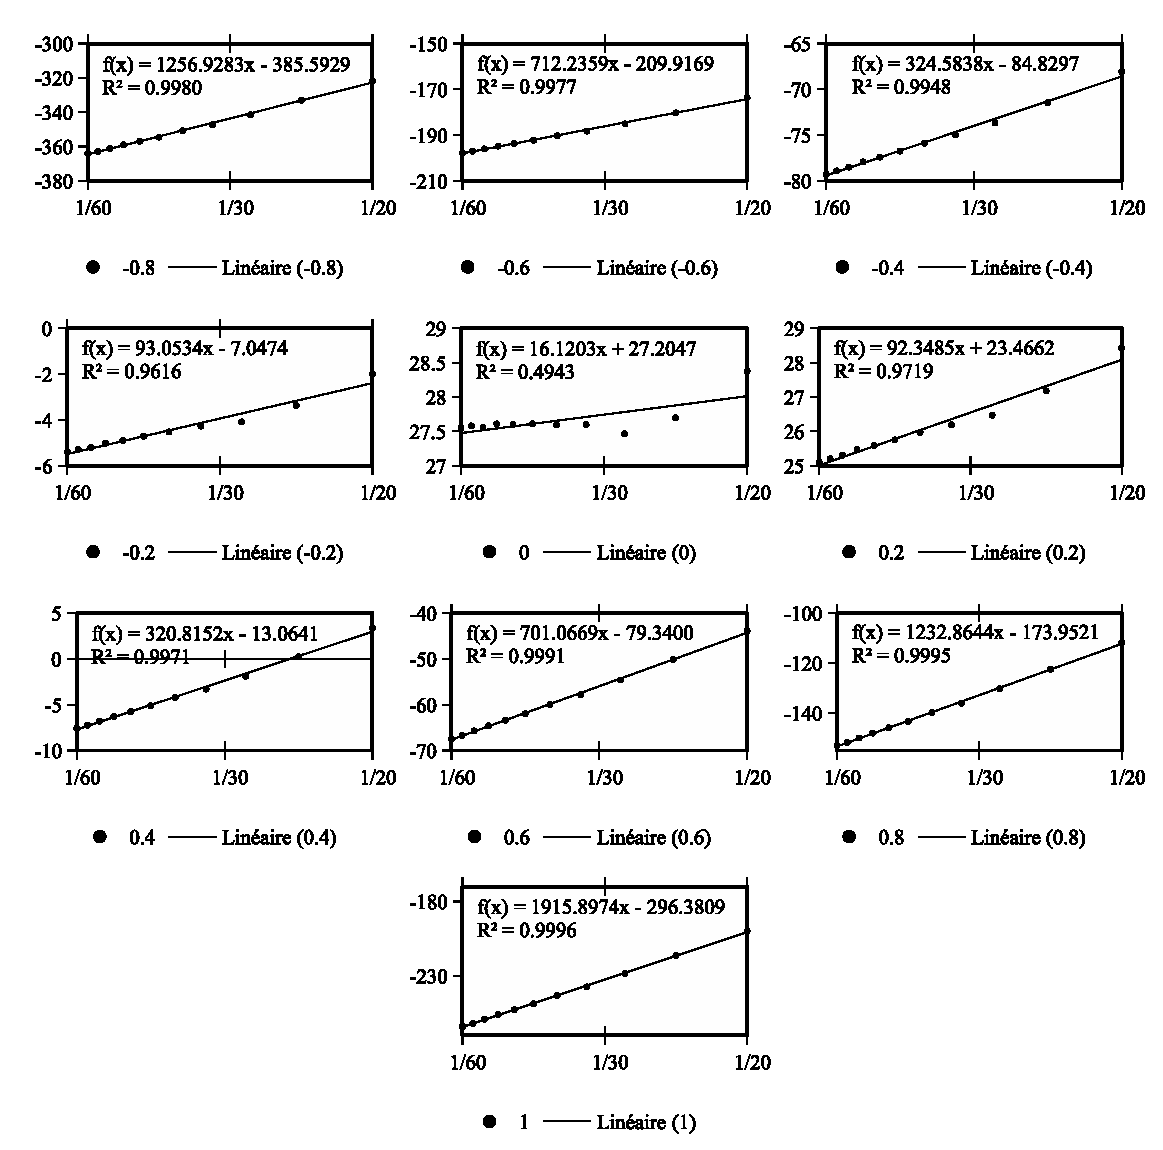
\includegraphics[width=0.95\columnwidth]{_figure/results/ch4_nmax1_lmn}
\par\end{centering}
\caption[Original free energy of charged $\mathrm{C}\mathrm{H}_{4}$, ``naive\_nmax1'']{Free energy (without correction) of charged $\mathrm{C}\mathrm{H}_{4}$
center (-1.0 to 1.0) with respect to the box length, for \texttt{\textbf{naive\_nmax1}}
method, with 6 angles of Lebedev quadrature angles for $\Theta$ and
$\Phi$, 3 for $\Psi$, DCF of $n_{\max}=1$, at 300K.\label{fig:ch4_nmax1_lmn}}
\end{figure}

\begin{figure}[!tbph]
\begin{centering}
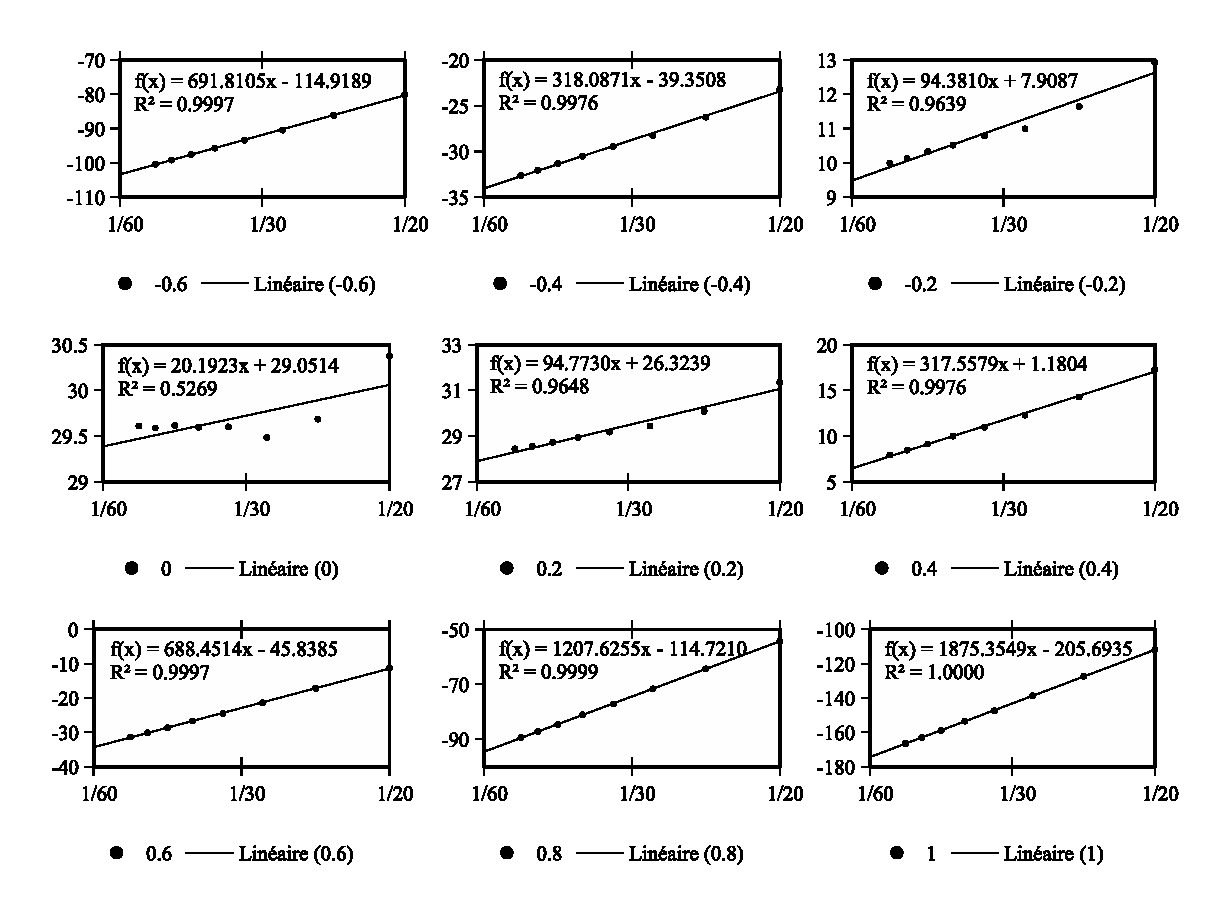
\includegraphics[width=0.95\columnwidth]{_figure/results/ch4_nmax5_inter}
\par\end{centering}
\caption[Original free energy of charged $\mathrm{C}\mathrm{H}_{4}$, ``naive\_interpolation''
with DCF of $n_{\max}=5$]{Free energy (without correction) of charged $\mathrm{C}\mathrm{H}_{4}$
center (-1.0 to 1.0) with respect to the box length, for \texttt{\textbf{naive\_interpolation}}
method, with 14 angles of Lebedev quadrature angles for $\Theta$
and $\Phi$, 3 for $\Psi$, DCF of $n_{\max}=5$, at 300K.\label{fig:ch4_nmax5_inter}}

\vspace{0.33cm}

\begin{centering}
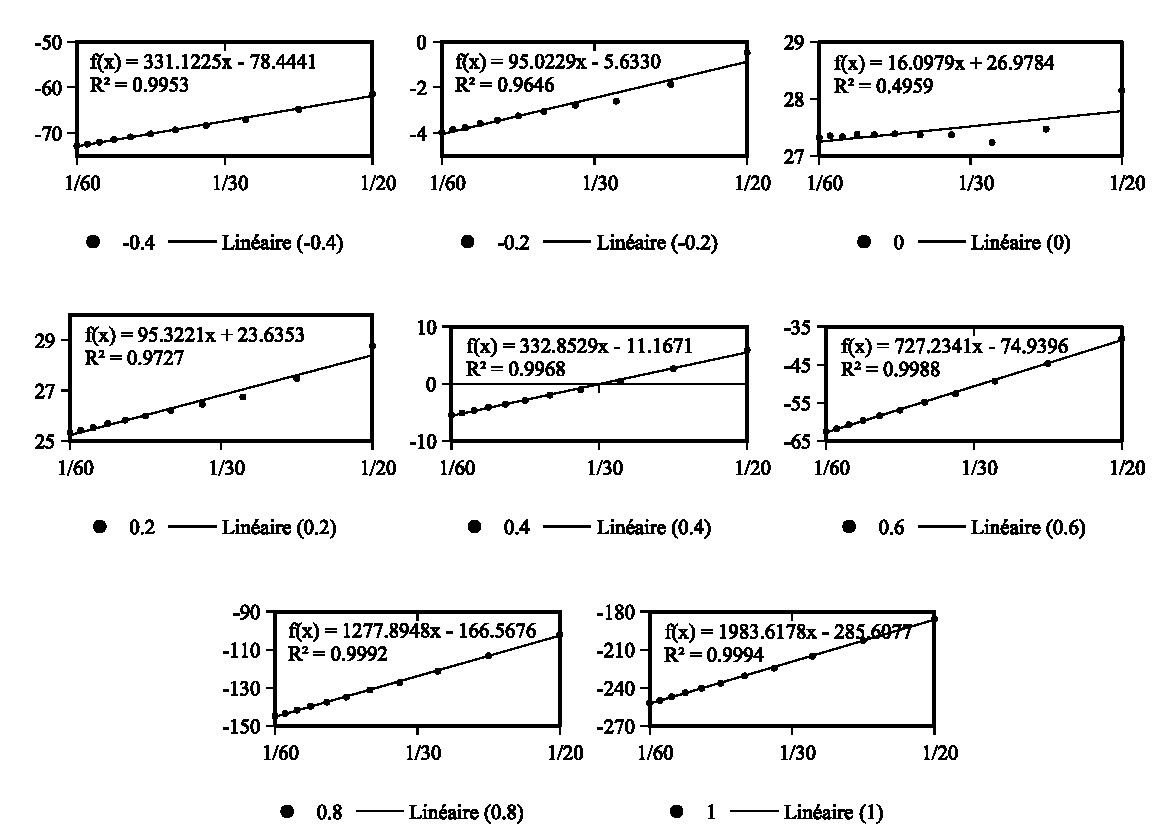
\includegraphics[width=0.95\columnwidth]{_figure/results/ch4_nmax1_new}
\par\end{centering}
\caption[Original free energy of charged $\mathrm{C}\mathrm{H}_{4}$, ``convolution\_standard''
with DCF of $n_{\max}=1$]{Free energy (without correction) of charged $\mathrm{C}\mathrm{H}_{4}$
center (-1.0 to 1.0) with respect to the box length, for \texttt{\textbf{convolution\_standard}}
method, with $m_{\max}=n_{\max}=1$, at 298.15K.\label{fig:ch4_nmax1_new}}
\end{figure}

The collections of the raw results issued directly from the code MDFT
are shown in figure \ref{fig:ch4_nmax1_lmn}, \ref{fig:ch4_nmax5_inter}
and \ref{fig:ch4_nmax1_new}. We can see that the dependence of box
length for each charge is almost linear, except for the charge between
$\left[-0.2,0.2\right]$ (where grid dependence dominated compared
to other effects). This means the influence of box length is much
greater than the intrinsic variation of result mentioned in \ref{sec:Intrinsic-variation-of}.
The charge dependency of the slopes in these figures is traced in
figure \ref{fig:Quadratic-charge-dependence} with respect to $\mathfrak{q}^{2}$,
square of the corresponding number charge. A linear regression is
done to give the slope in figure \ref{fig:Quadratic-charge-dependence}
at 1937.8 $\mathrm{kJ}\cdot\mathrm{mol^{-1}}\cdot\textrm{Å}$. This
slope corresponds to the correction of type-B:
\begin{equation}
\dfrac{f_{Q}\xi}{2}\left(1-\dfrac{1}{\varepsilon}\right)=1943.2\,\mathrm{kJ}\cdot\mathrm{mol^{-1}}\cdot\textrm{Å}
\end{equation}
where $f_{Q}=q_{e}^{2}10^{-3}N_{\mathrm{A}}/(4\pi\varepsilon_{0}10^{-10})$
is the electrostatic potential unit so that $f_{Q}\cdot\mathfrak{q}^{2}/r$
is in {[}$\mathrm{kJ\cdot mol^{-1}}${]}.

\begin{figure}[!th]
\begin{centering}
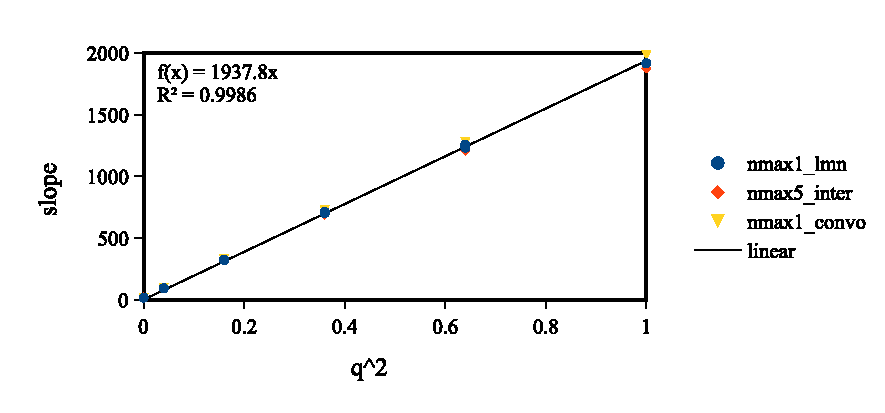
\includegraphics[bb=0bp 20bp 425bp 178bp,scale=0.75]{_figure/results/ch4_slope}
\par\end{centering}
\caption{Quadratic charge dependence of free energy in $\mathrm{C}\mathrm{H}_{4}^{\mathfrak{q}}$
series\label{fig:Quadratic-charge-dependence}}

\begin{centering}
\vspace{0.33cm}
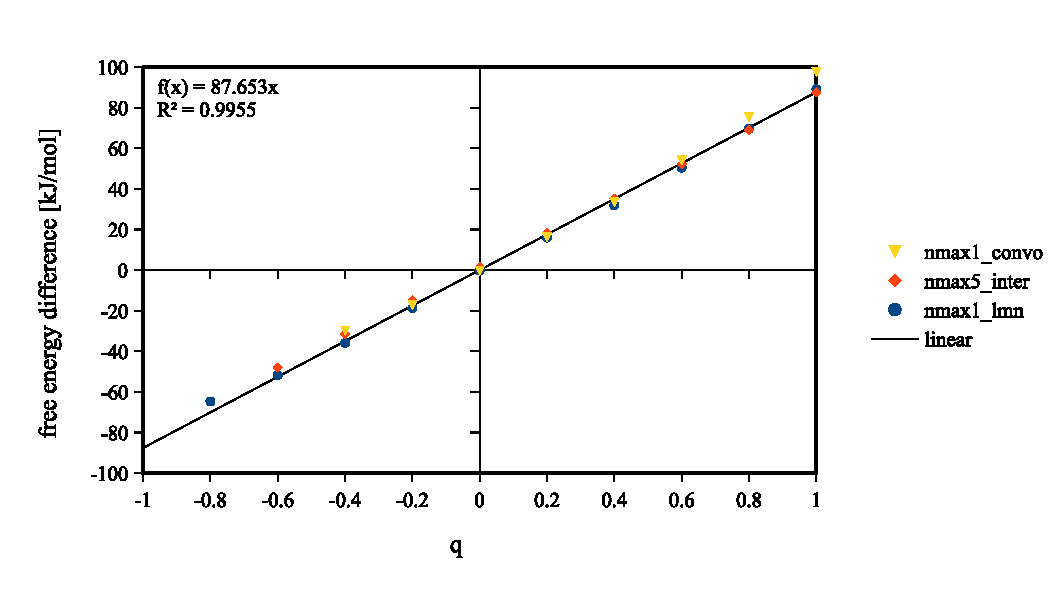
\includegraphics[bb=0bp 20bp 510bp 263bp,scale=0.75]{_figure/results/ch4_diff_energy}
\par\end{centering}
\caption[Free energy of charged $\mathrm{C}\mathrm{H}_{4}$ compared to \acs{IET},
without P-scheme correction]{Free energy (extrapolated to infinite box length) of charged $\mathrm{C}\mathrm{H}_{4}$
compared to \acs{IET}, without P-scheme correction\label{fig:Comparison-to-IET,without-correction}}
\end{figure}
The intercept values in each of figures \ref{fig:ch4_nmax1_lmn} to
\ref{fig:ch4_nmax1_new} correspond to the free energy of an infinite
box. The \acs{IET} results to be compared were obtained using the
1D-HNC formalism (1 distance, 5 angles) developed by Belloni and collaborators
\citep{belloni_efficient_2014}. The calculation were done with a
cut-off distance of $R_{\max}=102.4\textrm{Å}$ and an additional
Born-like correction of $-2.556k_{\mathrm{B}}T$ to obtain the free
energy in the infinite system. The difference in free energy between
\acs{MDFT} and \acs{IET} of the infinite system are given in figure
\ref{fig:Comparison-to-IET,without-correction}. The linear regression
is done with all existing points in this figure, and its slope 87.653
$\mathrm{kJ}\cdot\mathrm{mol^{-1}}$ corresponds to the correction
of type-C:
\begin{equation}
\dfrac{2\pi}{3}f_{Q}\eta\gamma=82.104\mathrm{kJ}\cdot\mathrm{mol^{-1}}\label{eq:eta-gamma}
\end{equation}
The measured number and the theoretical one are a little different,
it can be principally due to the lack of point at the -1 charge side.

\subsection{Comparison with IET after corrections}

\begin{figure}[!th]
\begin{centering}
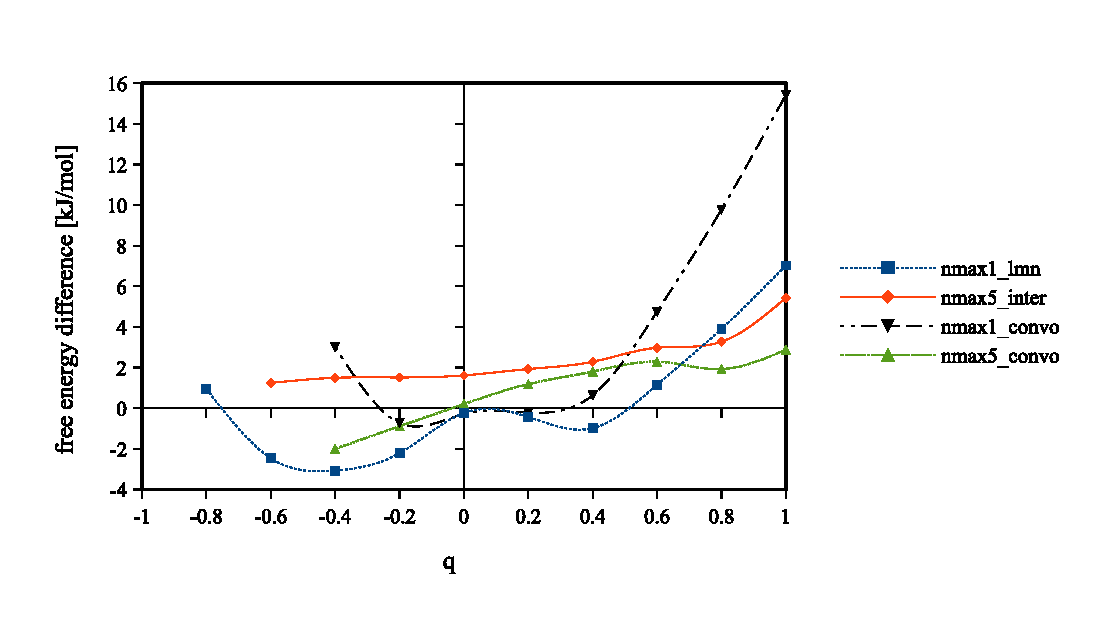
\includegraphics[bb=0bp 20bp 510bp 263bp,width=0.9\columnwidth]{_figure/results/ch4_diff_inter}
\par\end{centering}
\caption{Free energy difference of $\mathrm{C}\mathrm{H}_{4}^{\mathfrak{q}}$
series compared to IET, with all corrections\label{fig:Comparison-to-IET,with-corr}}

\begin{centering}
\vspace{0.33cm}
\par\end{centering}
\begin{centering}
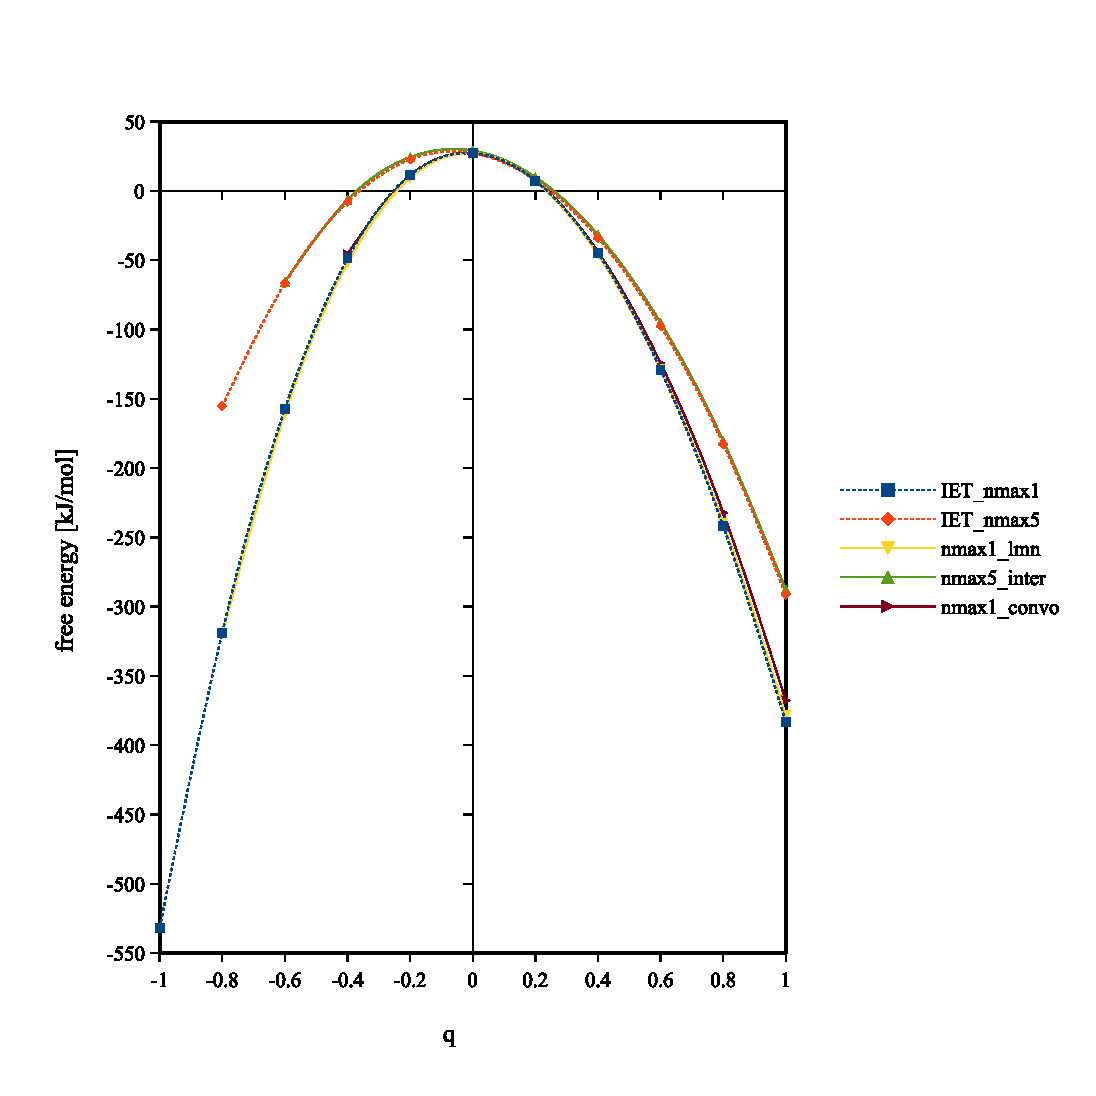
\includegraphics[bb=0bp 20bp 510bp 490bp,width=0.9\columnwidth]{_figure/results/ch4_inter_alles}
\par\end{centering}
\caption{Free energy of $\mathrm{C}\mathrm{H}_{4}^{\mathfrak{q}}$ series,
with all corrections\label{fig:Comparison-to-IET,with-corr-alles}}
\end{figure}

The points in figure \ref{fig:Comparison-to-IET,without-correction}
after correction with eq. (\ref{eq:eta-gamma}), as well as the difference
between results of $m_{\max}=n_{\max}=5$ given by \texttt{\textbf{convolution\_standard}}
(with $L=24$ $\textrm{Å}$, $\mathrm{nfft}=72$) using theoretical
corrections and \acs{IET} with infinite corrections (nmax5\_convo)
are shown in figure \ref{fig:Comparison-to-IET,with-corr}. Note that
the curves for the same \acs{DCF} are not perfectly in agreement
with each other, despite what is shown in table \ref{tab:free-energy}.
The fact is that in ``nmax1\_lmn'', Lebedev quadrature is used,
and in ``nmax1\_convo'', Gauss-Legendre quadrature is used, as we
know the different angular grid can have an effect on the energy;
and for $n_{\max}=5$, as we have taken by chance the +0.4 as charge
in table \ref{tab:free-energy}, the difference between the \texttt{\textbf{naive\_interpolation}}
and \texttt{\textbf{convolution\_standard}} results are accidentally
small. The troublesome energy shift of about 2 $\mathrm{kJ}\cdot\mathrm{mol^{-1}}$
between ``nmax5\_inter'' and \acs{IET} result is yet to be understood,
as well as the dependence on $q$ for ``nmax5\_convo'' after correction.
But if we look at the free energies without comparing them in figure
\ref{fig:Comparison-to-IET,with-corr-alles}, we can see that these
differences are almost negligible compared to the total energy they
possess, and the curves only differs with different \acs{DCF}s.

\subsection{Dependence on $m_{\max}$ and $n_{\max}$}

\begin{table}
\begin{centering}
\begin{tabular*}{1\linewidth}{@{\extracolsep{\fill}}cccccccccc}
\toprule 
\addlinespace[-0.17em]
\tableheadline{{\footnotesize{}Charge}} & \multicolumn{3}{c}{{\scriptsize{}-0.6}} & \multicolumn{3}{c}{{\scriptsize{}0}} & \multicolumn{3}{c}{{\scriptsize{}1}}\tabularnewline
\midrule 
\addlinespace[-0.33em]
{\scriptsize{}$n_{\max}$\textbackslash{}$m_{\max}$} & {\scriptsize{}IET} & {\scriptsize{}$=n_{\max}$} & {\scriptsize{}$=5$} & {\scriptsize{}IET} & {\scriptsize{}$=n_{\max}$} & {\scriptsize{}$=5$} & {\scriptsize{}IET} & {\scriptsize{}$=n_{\max}$} & {\scriptsize{}$=5$}\tabularnewline
\midrule 
\addlinespace[-0.33em]
{\scriptsize{}1} & {\scriptsize{}-157.48} & {\scriptsize{}diverge} & {\scriptsize{}-163.35} & {\scriptsize{}27.33} & {\scriptsize{}27.47} & {\scriptsize{}27.97} & {\scriptsize{}-382.34} & {\scriptsize{}-365.89} & {\scriptsize{}-379.01}\tabularnewline
\addlinespace[-0.33em]
{\scriptsize{}2} & {\scriptsize{}-84.32} & {\scriptsize{}-87.56} & {\scriptsize{}-87.71} & {\scriptsize{}27.82} & {\scriptsize{}27.94} & {\scriptsize{}28.12} & {\scriptsize{}-301.74} & {\scriptsize{}-298.95} & {\scriptsize{}-298.67}\tabularnewline
\addlinespace[-0.33em]
{\scriptsize{}3} & {\scriptsize{}-66.25} & {\scriptsize{}-69.58} & {\scriptsize{}-69.70} & {\scriptsize{}27.16} & {\scriptsize{}27.24} & {\scriptsize{}27.50} & {\scriptsize{}-294.77} & {\scriptsize{}-292.12} & {\scriptsize{}-291.87}\tabularnewline
\addlinespace[-0.33em]
{\scriptsize{}4} & {\scriptsize{}no data} & {\scriptsize{}-69.41} & {\scriptsize{}-69.50} & {\scriptsize{}no data} & {\scriptsize{}27.85} & {\scriptsize{}27.91} & {\scriptsize{}no data} & {\scriptsize{}-289.19} & {\scriptsize{}-289.04}\tabularnewline
\addlinespace[-0.33em]
{\scriptsize{}5} & {\scriptsize{}-66.50} & {\scriptsize{}diverge} & {\scriptsize{}diverge} & {\scriptsize{}27.25} & {\scriptsize{}27.47} & {\scriptsize{}27.47} & {\scriptsize{}-291.60} & {\scriptsize{}-288.54} & {\scriptsize{}-288.54}\tabularnewline
\bottomrule
\end{tabular*}
\par\end{centering}
\caption[Free energy of $\mathrm{C}\mathrm{H}_{4}^{\mathfrak{q}}$ series (with
corrections) for different $m_{\max}$ and $n_{\max}$]{Free energy of $\mathrm{C}\mathrm{H}_{4}^{\mathfrak{q}}$ series
(with corrections) for \acs{IET}, $m_{\max}=n_{\max}$ and $m_{\max}=5$,
using \texttt{\textbf{convolution\_standard}}, with $L=24$ $\textrm{Å}$,
$\mathrm{nfft}=72$.\label{tab:Free-energy-of-mnmax}}
\end{table}
\begin{figure}[!th]
\begin{centering}
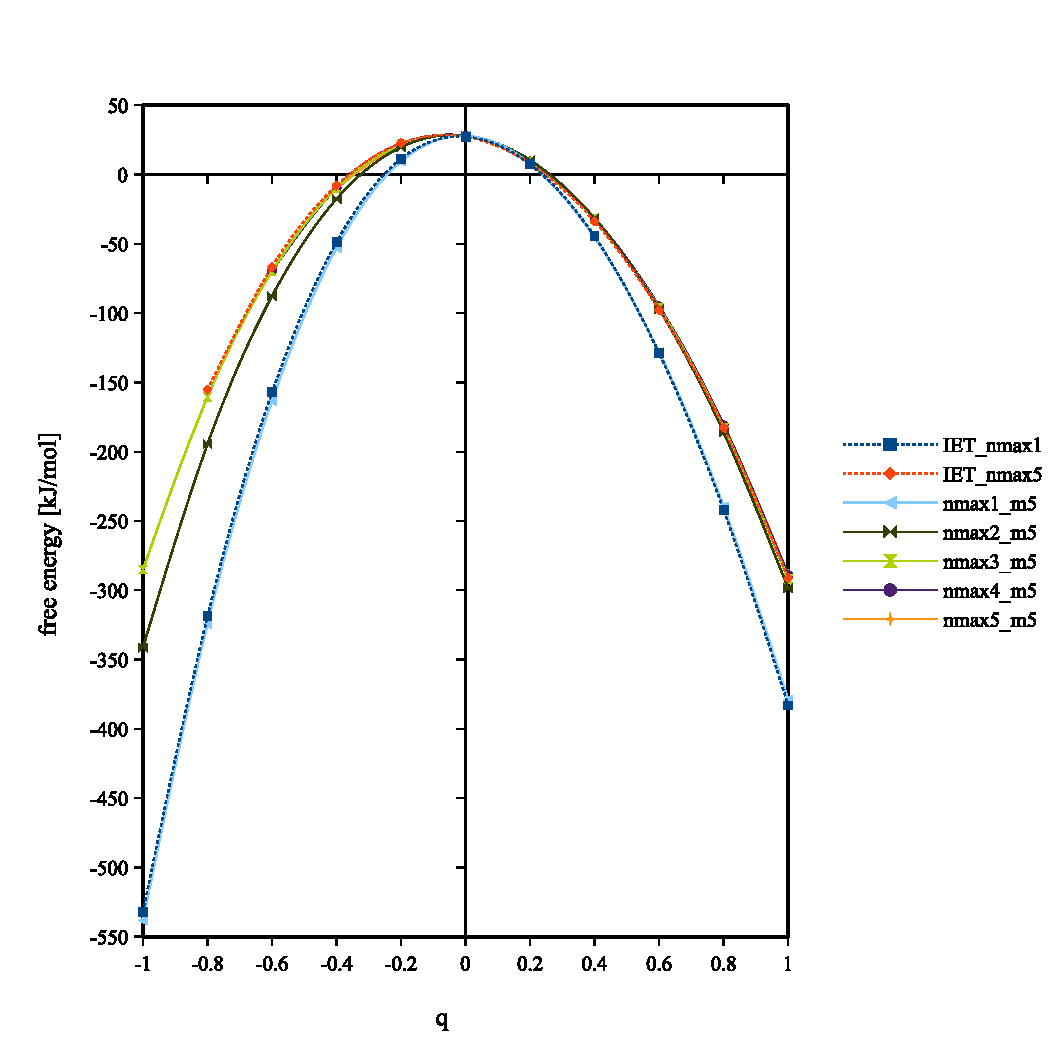
\includegraphics[bb=0bp 20bp 510bp 490bp,width=0.9\columnwidth]{_figure/results/ch4_inter_nmax}
\par\end{centering}
\caption[Free energy of $\mathrm{C}\mathrm{H}_{4}^{\mathfrak{q}}$ series (with
corrections) for different $n_{\max}$ ($m_{\max}=5$)]{Free energy of $\mathrm{C}\mathrm{H}_{4}^{\mathfrak{q}}$ series,
with all corrections of \acs{IET} results and \acs{MDFT} $m_{\max}=5$,
$n_{\max}=0,\ldots,5$.\label{fig:Comparison-to-IET,with-corr-nmax}}
\end{figure}

As we see, the free energy of charged $\mathrm{C}\mathrm{H}_{4}^{\mathfrak{q}}$
series depends a lot on the order of \acs{DCF}, $n_{\max}$. To study
systematically the influence of $m_{\max}$ and $n_{\max}$, we chose
a series of tests with three charge: -0.6, 0, and +1, using \texttt{\textbf{convolution\_standard}},
as shown in table \ref{tab:Free-energy-of-mnmax}. Three types of
energy are listed: the results issued from \acs{IET}, the case when
$m_{\max}=n_{\max}$ and $m_{\max}=5$. As we said previously the
gradient $\gamma$ is smoother than $\rho$; it is worthwhile to study
the case when the order of quadrature $m_{\max}$ for the expansion
of $\rho$ is larger than the order of \acs{DCF} $n_{\max}$ used
in equation \acs{OZ} to solve $\gamma$, in order to save computing
cost.

From table \ref{tab:Free-energy-of-mnmax} we can see that the free
energy becomes stable in any case when $n_{\max}\geq3$; the free
energies are quite in agreement with \acs{IET} results; and there
is almost no difference between $m_{\max}=n_{\max}$ and $m_{\max}=5$.
That means, the quadrature of $\rho$ have no influence to the final
energy, which is yet comprehensible, as the extra order of quadrature
gives no influence to the functional gradient, and the $\rho$ used
to evaluate the functional is given by minimization, i.e. without
expansion on \acs{GSH}s.

A scheme of free energy evaluation with respect to $n_{\max}$ ($m_{\max}=5$,
as some of the points of $m_{\max}=n_{\max}$ have difficulty to converge
and if convergence is achieved they give usually the same result)
is made in figure \ref{fig:Comparison-to-IET,with-corr-nmax}. We
see that from $n_{\max}=3$ to higher order, the curves do not vary
a lot. We can conclude that within $n_{\max}\geq3$ to $n_{\max}=5$,
the error in free energy is acceptable.\marginpar{We take solute-solvent formalism for \acs{MDFT}, and \acs{IET} takes
the solvent-solute formalism. Thus in \acs{MDFT} the $g_{\mu\nu}^{mnl}$
corresponds to the $g_{\nu\mu}^{nml}$ in \acs{IET}. In figure \ref{fig:Comparison-to-IET.rot_invar}
it is converted to give a easier understanding. }

Some selected projections $\rho_{0\nu}^{0nl}(r)$ (0 as solute is
spherical) are compared to \acs{IET} in figure \ref{fig:Comparison-to-IET.rot_invar}.
We can see that they are in good agreement.

\begin{figure}[!t]
\begin{centering}
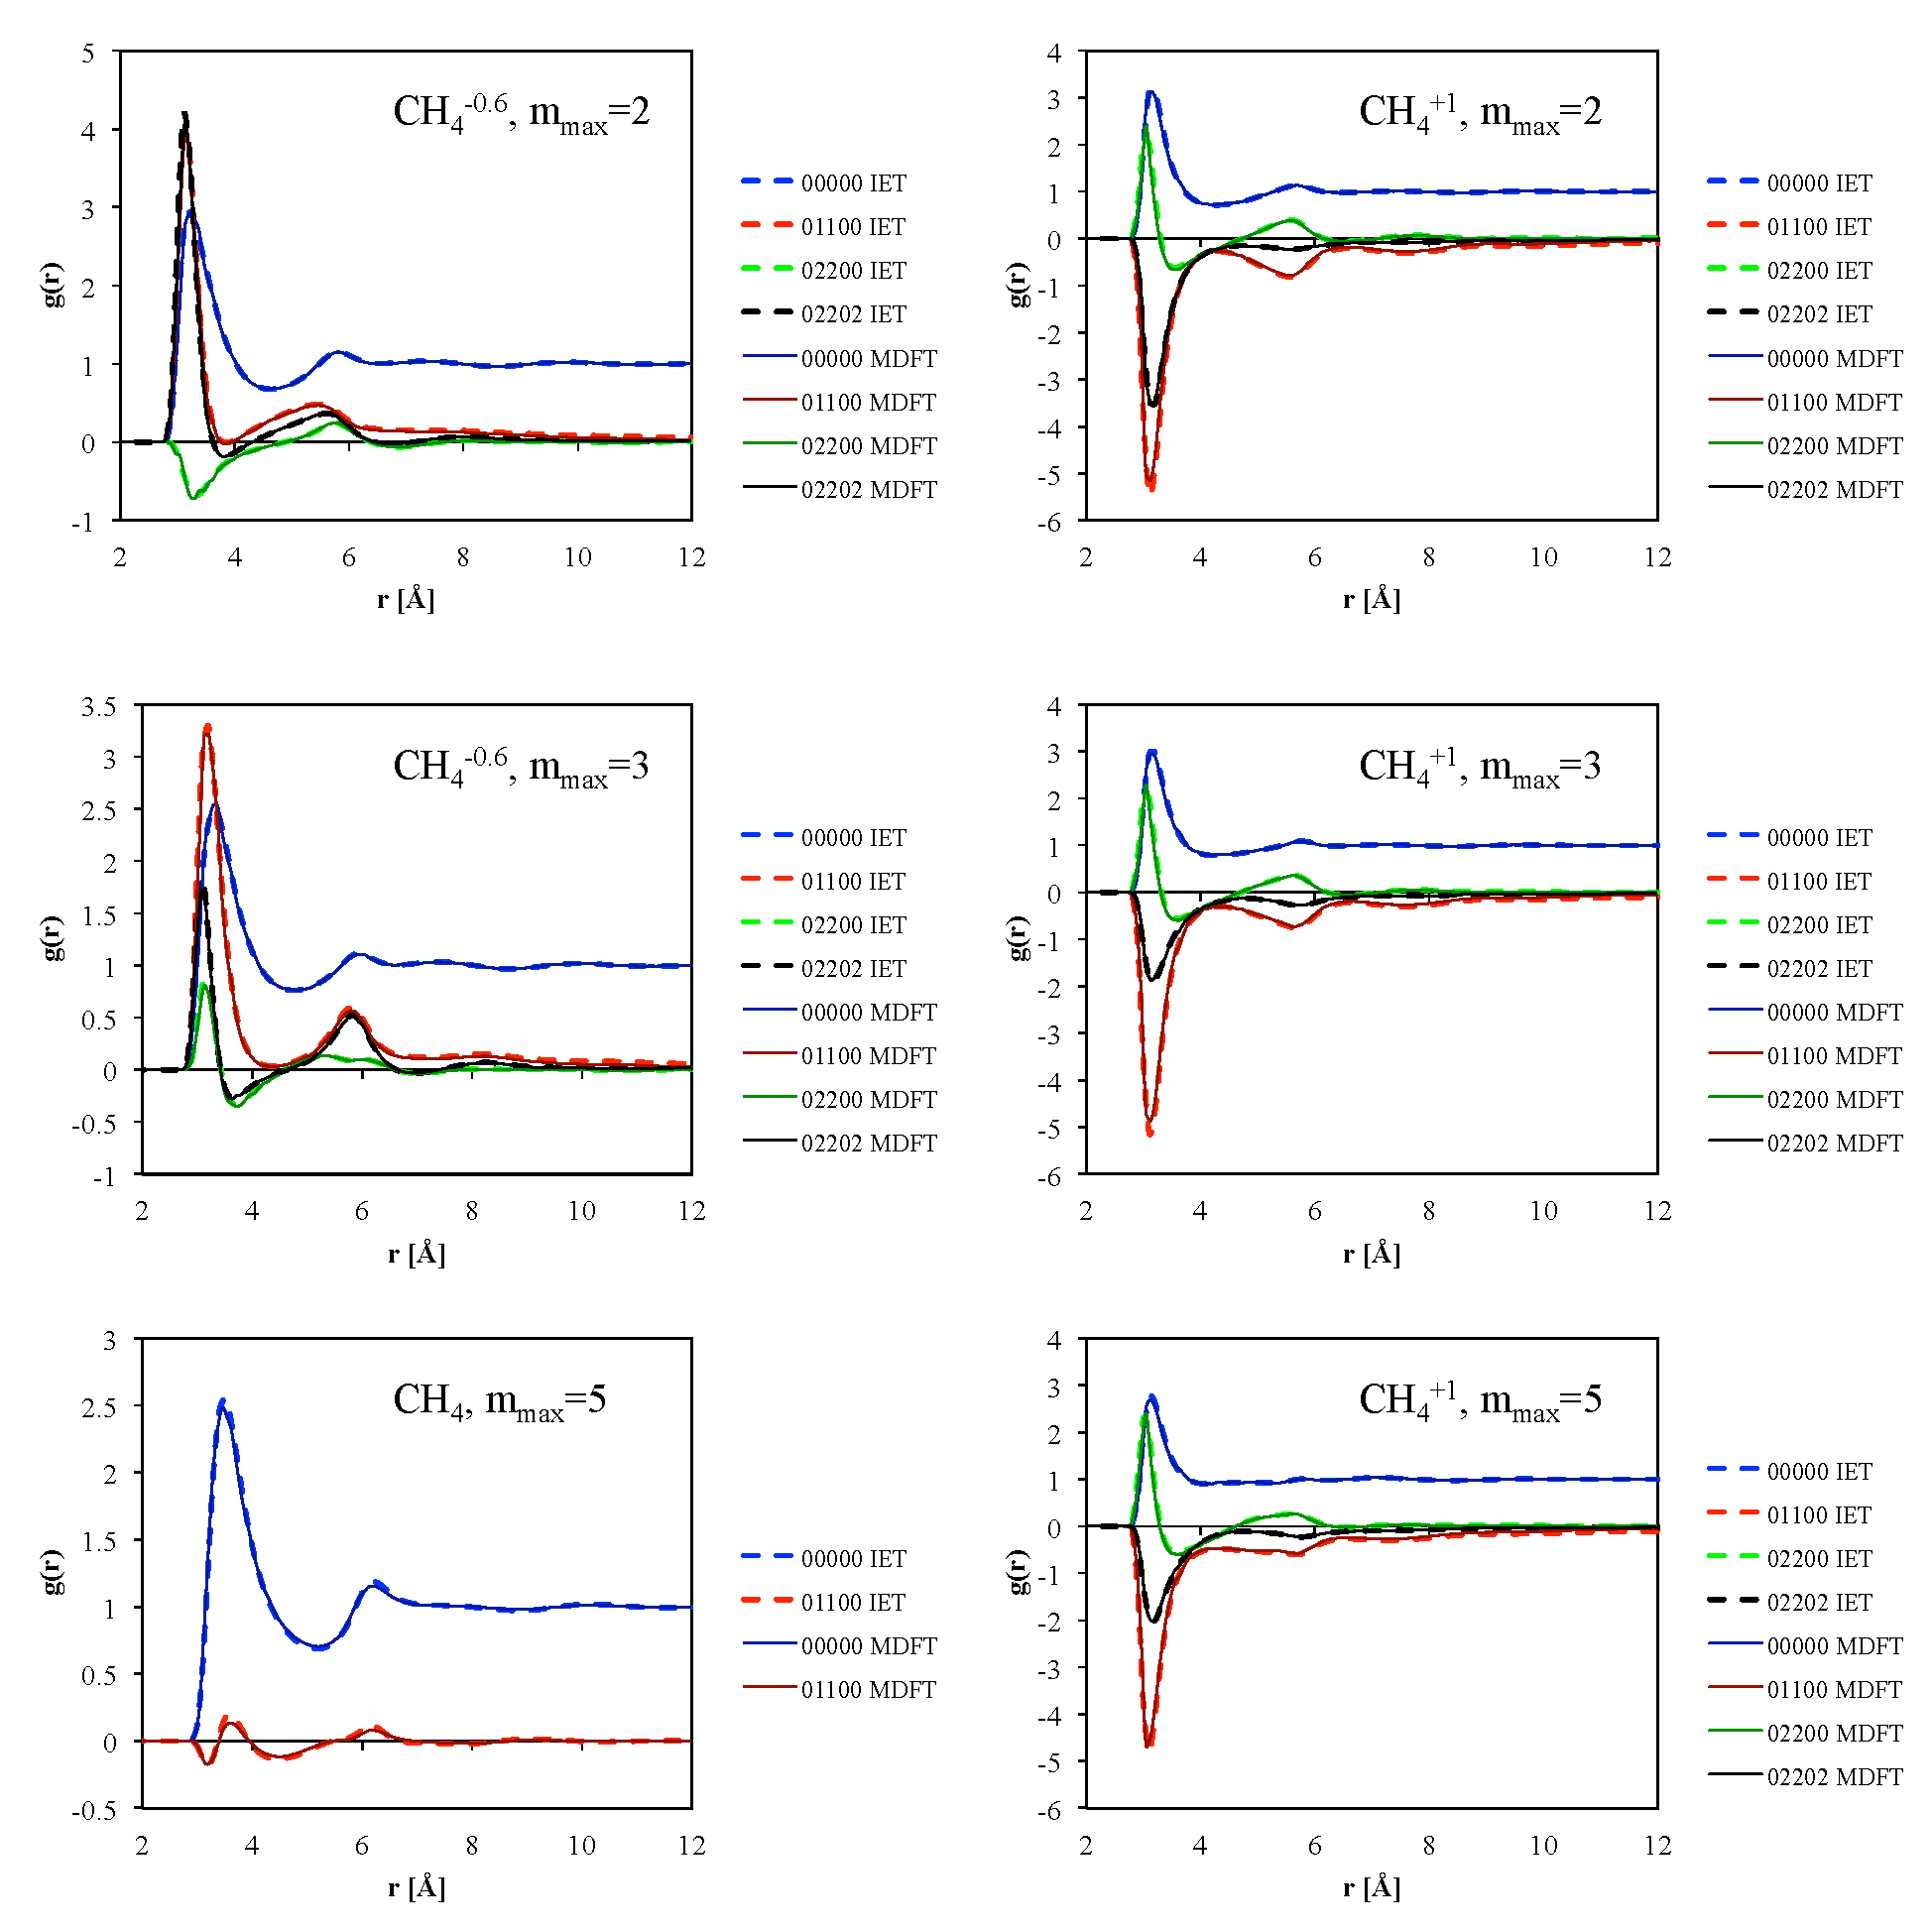
\includegraphics[width=1\columnwidth]{_figure/results/ch4_iet_struct}
\par\end{centering}
\caption[The projections $\rho_{0\nu}^{0nl}(r)$ of some selected charges of
$\mathrm{C}\mathrm{H}_{4}^{\mathfrak{q}}$ series comparing to \acs{IET}]{The projections $\rho_{0\nu}^{0nl}(r)$ of some selected charges
of $\mathrm{C}\mathrm{H}_{4}^{\mathfrak{q}}$ series comparing to
\acs{IET}, with $m_{\max}=n_{\max}$.\label{fig:Comparison-to-IET.rot_invar}}
\end{figure}

\begin{figure}[!th]
\begin{centering}
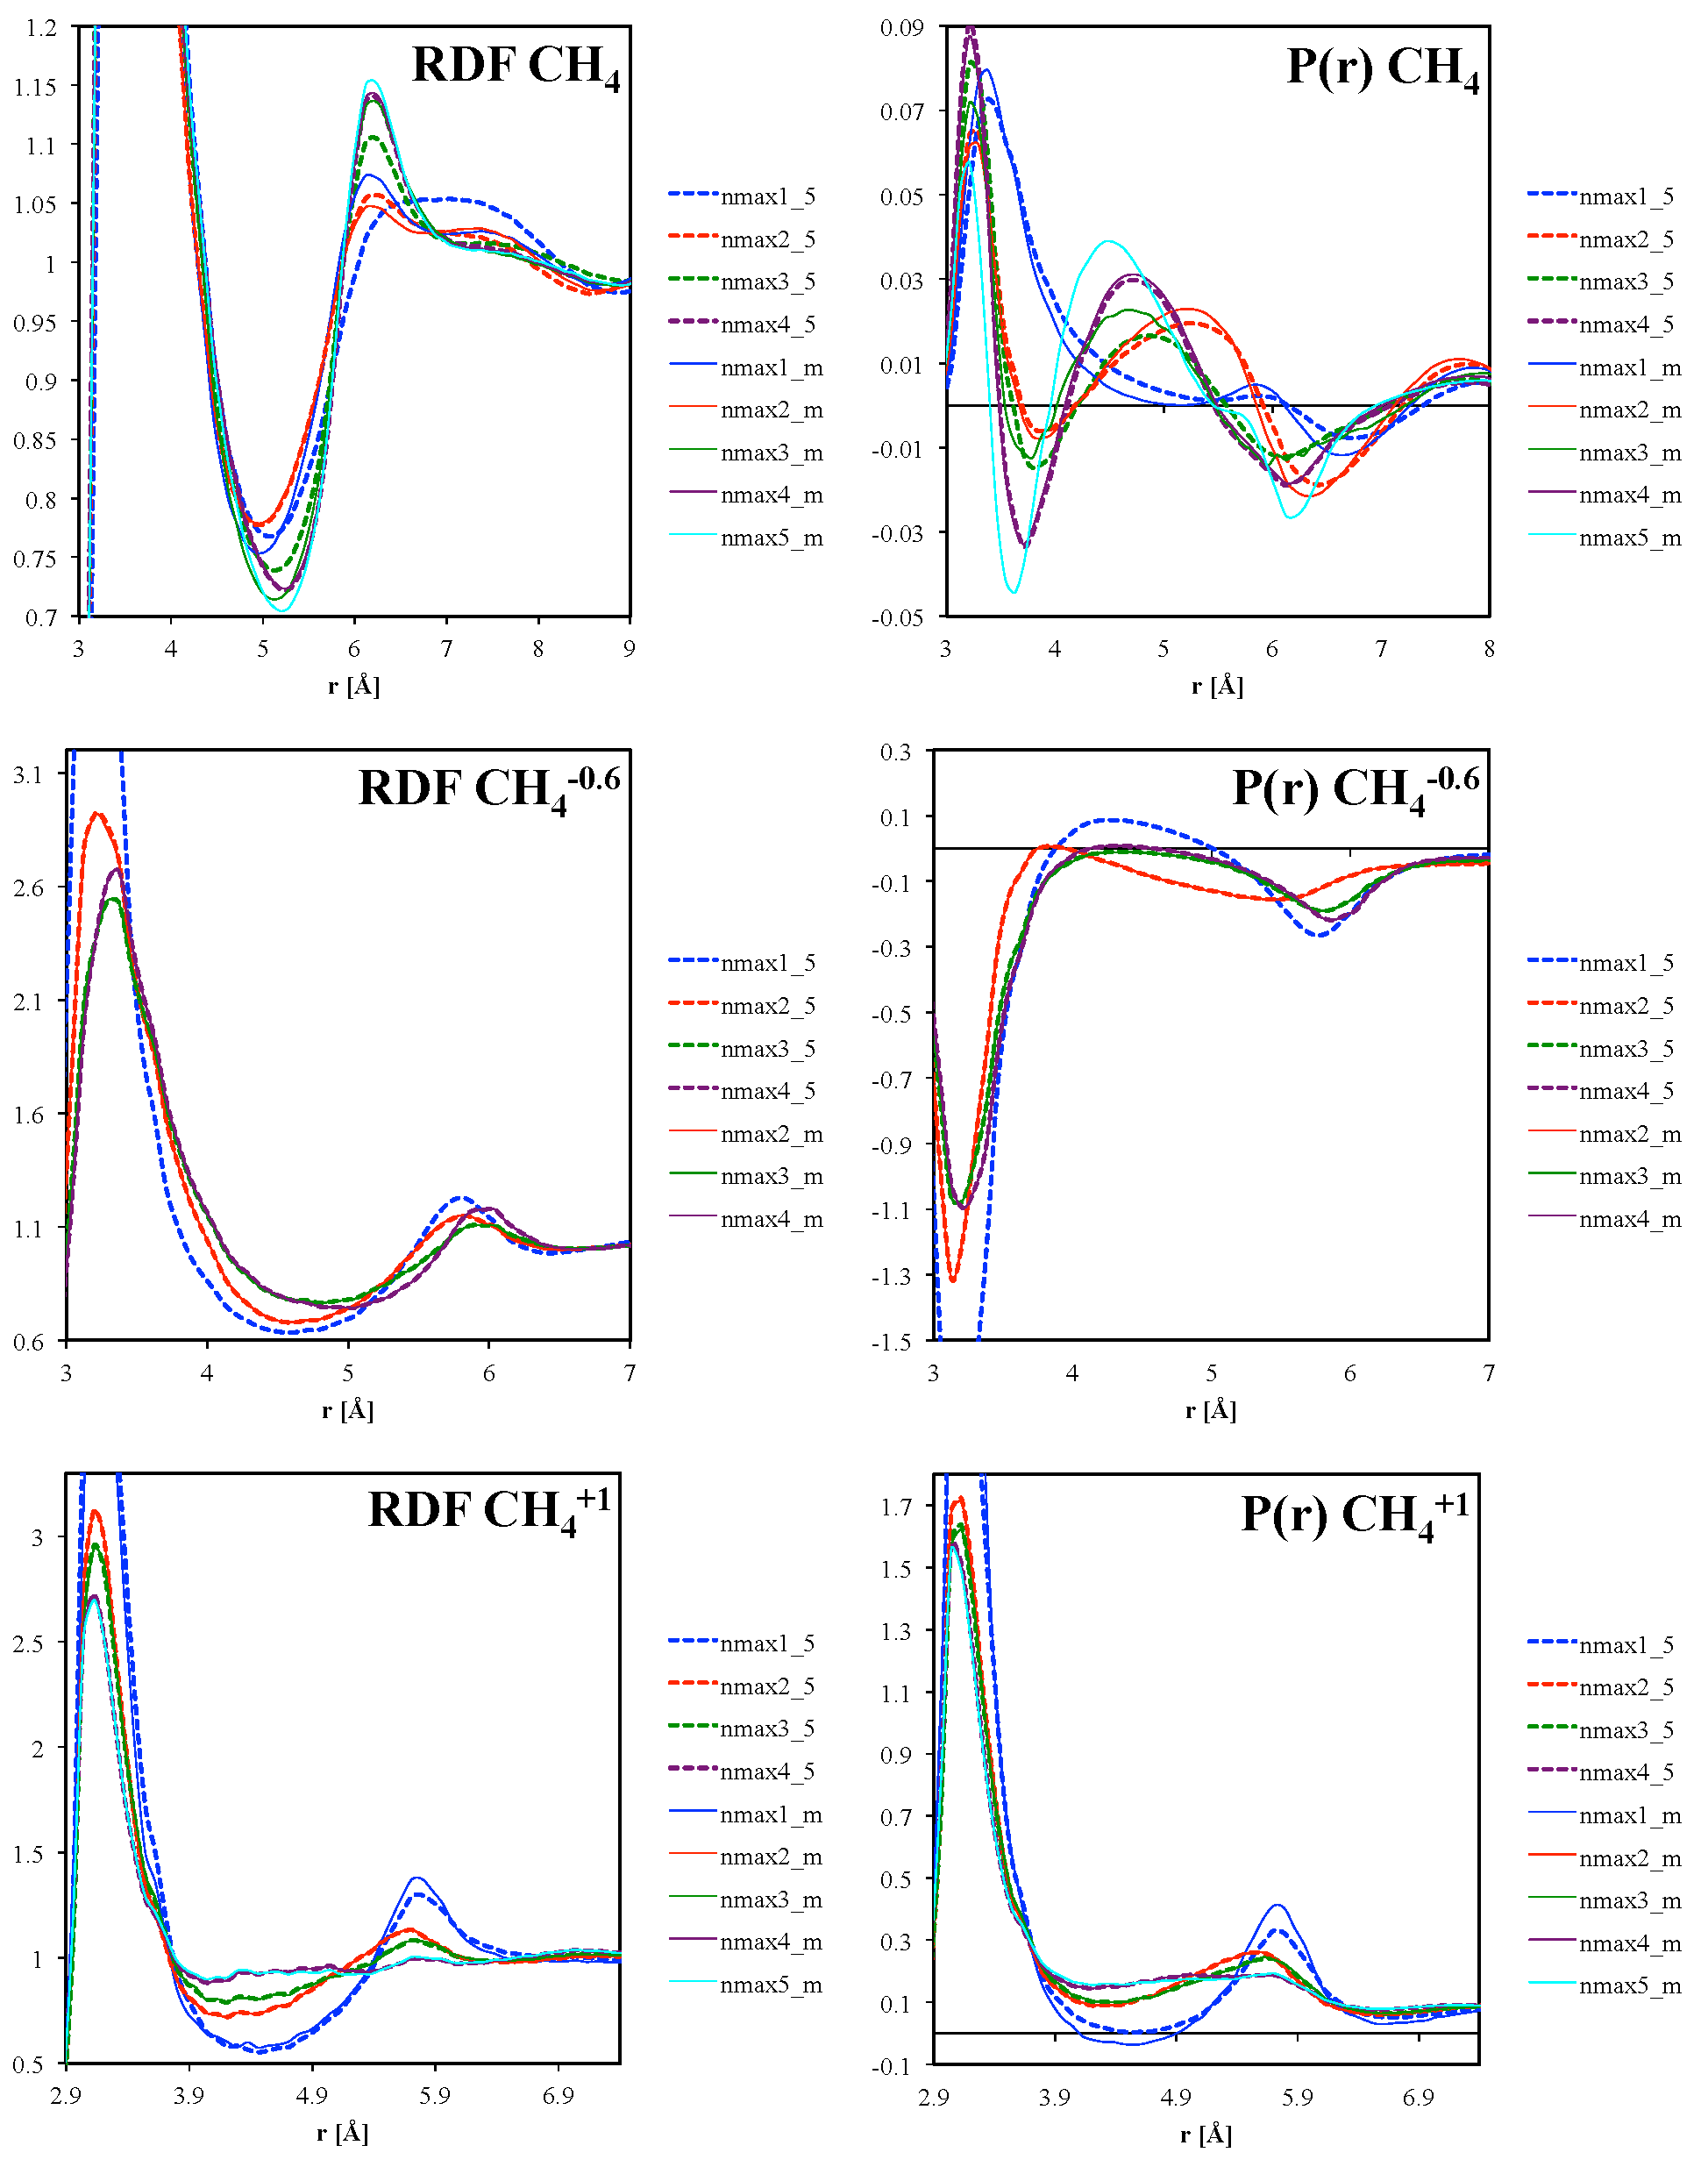
\includegraphics[width=1\columnwidth]{_figure/results/ch4_series}
\par\end{centering}
\caption{\acs{RDF} and \acs{RPF} of some selected charges of $\mathrm{C}\mathrm{H}_{4}^{\mathfrak{q}}$
series with different $m_{\max}$ and $n_{\max}$\label{fig:RDF-and-polarization}}
\end{figure}

If we compare one charge in one graph, with all the $n_{\max}$, we
can determine which $n_{\max}$ is sufficient to have a good structure
of the density $\rho$. Figure \ref{fig:RDF-and-polarization} gives
the \acs{RDF}s and \acs{RPF}s for the three charges, as well as
their zoomed parts in order to have a clear view of the differences.
Firstly we can see that in the most of cases, apart form uncharged
$\mathrm{C}\mathrm{H}_{4}$ and some $n_{\max}=1$, the curves of
$m_{\max}=5$ and $m_{\max}=n_{\max}$ are superposed. That means
even for structure of single ions, extra order of $m_{\max}$ is useless.
For -0.6, the curves converge from $n_{\max}=3$, and for +1, $n_{\max}=4$.
For $\mathrm{C}\mathrm{H}_{4}$ it seems to be bazar, but looking
at the scale of the schema and we consider that it converges from
$n_{\max}=4$. To conclude, for $\mathrm{C}\mathrm{H}_{4}^{\mathfrak{q}}$
series, we think $n_{\max}=3$ is sufficient for energy, and $n_{\max}=4$
is sufficient for the structure to converge (without considering higher
order projections).

\section{Uncharged LJ centers}

As there is an energy shift between \texttt{\textbf{naive\_interpolation}}
and \acs{IET} results even for un charged $\mathrm{C}\mathrm{H}_{4}$
(figure \ref{fig:Comparison-to-IET,with-corr}), we have calculated
in addition some other uncharged LJ centers. 
\begin{table}[h]
\begin{centering}
\begin{tabular*}{1\linewidth}{@{\extracolsep{\fill}}ccccccccccc}
\toprule 
\addlinespace[-0.17em]
\tableheadline{{\footnotesize{}Solute}} & {\scriptsize{}$\sigma$} & {\scriptsize{}$\epsilon$} & {\scriptsize{}dipole} & {\scriptsize{}1} & {\scriptsize{}2} & {\scriptsize{}3} & {\scriptsize{}4} & {\scriptsize{}5} & {\scriptsize{}inter} & {\scriptsize{}IET}\tabularnewline
\midrule 
\addlinespace[-0.33em]
{\scriptsize{}Neon} & {\scriptsize{}3.035} & {\scriptsize{}0.15432} & {\scriptsize{}18.61} & {\scriptsize{}18.79} & {\scriptsize{}19.03} & {\scriptsize{}18.56} & {\scriptsize{}18.99} & {\scriptsize{}18.86} & {\scriptsize{}20.04} & {\scriptsize{}18.82}\tabularnewline
\addlinespace[-0.33em]
{\scriptsize{}Argon} & {\scriptsize{}3.415} & {\scriptsize{}1.03931} & {\scriptsize{}22.16} & {\scriptsize{}22.47} & {\scriptsize{}22.86} & {\scriptsize{}22.15} & {\scriptsize{}22.72} & {\scriptsize{}22.39} & {\scriptsize{}24.24} & {\scriptsize{}22.27}\tabularnewline
\addlinespace[-0.33em]
{\scriptsize{}Krypton} & {\scriptsize{}3.675} & {\scriptsize{}1.4051} & {\scriptsize{}25.36} & {\scriptsize{}25.76} & {\scriptsize{}26.23} & {\scriptsize{}25.48} & {\scriptsize{}26.14} & {\scriptsize{}25.73} & {\scriptsize{}27.82} & {\scriptsize{}25.49}\tabularnewline
\addlinespace[-0.33em]
{\scriptsize{}Xenon} & {\scriptsize{}3.975} & {\scriptsize{}1.7851} & {\scriptsize{}29.68} & {\scriptsize{}30.24} & {\scriptsize{}30.77} & {\scriptsize{}30.13} & {\scriptsize{}30.74} & {\scriptsize{}30.25} & {\scriptsize{}32.66} & {\scriptsize{}29.92}\tabularnewline
\bottomrule
\end{tabular*}
\par\end{centering}
\caption[Free energy of rare gases]{Free energy $[\mathrm{kJ\cdot mol^{-1}}]$ of rare gases, for respectively
\texttt{\textbf{reference\_dipole}}, \texttt{\textbf{convolution\_standard}}
with $m_{\max}=n_{\max}=1,\ldots,5$, and \texttt{\textbf{naive\_interpolation}}
with \acs{DCF} of $n_{\max}=5$; $\sigma$ in $[\textrm{Å}]$, $\epsilon$
in $[\mathrm{kJ\cdot mol^{-1}}]$, with $L=24$ $\textrm{Å}$, $\mathrm{nfft}=72$.\label{tab:Free-energy-rare-gas}}
\end{table}
Results in table \ref{tab:Free-energy-rare-gas} show that this energy
shift is common in any uncharged LJ centers; and in these cases, even
$n_{\max}=1$ can satisfy the requirement of chemical precision.

\section{Linear solutes}

To complete the story of $m_{\max}$ and $n_{\max}$ convergence,
we choose some linear solutes shown in figure \ref{fig:Test-linear-solutes}
and table \ref{tab:Parameters-of-test-solutes}. The direct summation
method ($\mathsection$\ref{subsec:The-external-term}) is used for
$\mathcal{F}_{\mathrm{ext}}$ evaluation, as $\mathrm{O}_{2}$ always
diverges with Poisson method. We can make hypothesis that this is
because the distance between the charges is too short, as shown in
figure \ref{fig:Test-linear-solutes}; therefore the interpolation
in $\mathcal{F}_{\mathrm{ext}}$ evaluation can cause divergence.
There is a better version of Poisson solver that is developed in parallel
of this code, which has been reported to have better convergency.
We consider that this divergency problem does not come from the evaluation
of $\mathcal{F}_{\mathrm{exc}}$.

\begin{figure}[h]
\begin{centering}
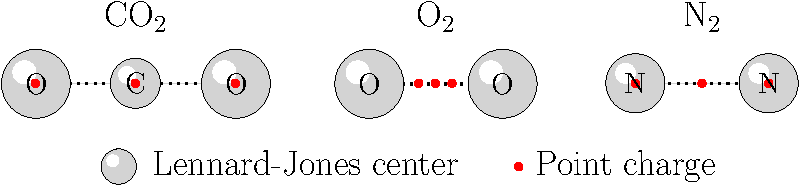
\includegraphics[scale=0.6]{_figure/app_solute}
\par\end{centering}
\caption{Test linear solutes\label{fig:Test-linear-solutes}}
\end{figure}

\begin{table}[h]
\begin{centering}
\begin{tabular*}{1\linewidth}{@{\extracolsep{\fill}}cccccc}
\toprule 
\addlinespace[-0.17em]
\tableheadline{{\footnotesize{}Solute}} & \tableheadline{{\footnotesize{}Site}} & {\scriptsize{}$q$} & {\scriptsize{}$\sigma$ $[\textrm{Å}]$} & {\scriptsize{}$\epsilon$ {[}$\mathrm{kJ\cdot mol^{-1}}${]}} & {\scriptsize{}$x$ $[\textrm{Å}]$}\tabularnewline
\midrule 
\addlinespace[-0.33em]
{\scriptsize{}$\mathrm{CO_{2}}$ \citep{Harris_1995}} & {\scriptsize{}1} & {\scriptsize{}0.6512 } & {\scriptsize{}2.76} & {\scriptsize{}0.234} & {\scriptsize{}0.000 }\tabularnewline
\addlinespace[-0.33em]
{\scriptsize{}(20.48 {[}$\mathrm{kJ\cdot mol^{-1}}${]})} & {\scriptsize{}2} & {\scriptsize{}-0.3256} & {\scriptsize{}3.03 } & {\scriptsize{}0.67} & {\scriptsize{}-1.149 }\tabularnewline
\addlinespace[-0.33em]
 & {\scriptsize{}3} & {\scriptsize{}-0.3256} & {\scriptsize{}3.03 } & {\scriptsize{}0.67} & {\scriptsize{}1.149 }\tabularnewline
\midrule 
\addlinespace[-0.33em]
{\scriptsize{}$\mathrm{O_{2}}$ \citep{Boutard200525}} & {\scriptsize{}1} & {\scriptsize{}0.0} & {\scriptsize{}3.1062} & {\scriptsize{}0.36 } & {\scriptsize{}-0.485}\tabularnewline
\addlinespace[-0.33em]
{\scriptsize{}(22.05 {[}$\mathrm{kJ\cdot mol^{-1}}${]})} & {\scriptsize{}2} & {\scriptsize{}0.0} & {\scriptsize{}3.1062} & {\scriptsize{}0.36 } & {\scriptsize{}0.485}\tabularnewline
\addlinespace[-0.33em]
 & {\scriptsize{}3} & {\scriptsize{}-2.1} & {\scriptsize{}0.00} & {\scriptsize{}0.00} & {\scriptsize{}-0.200}\tabularnewline
\addlinespace[-0.33em]
 & {\scriptsize{}4} & {\scriptsize{}-2.1} & {\scriptsize{}0.00} & {\scriptsize{}0.00} & {\scriptsize{}0.200}\tabularnewline
\addlinespace[-0.33em]
 & {\scriptsize{}5} & {\scriptsize{}4.2} & {\scriptsize{}0.00} & {\scriptsize{}0.00} & {\scriptsize{}0.000}\tabularnewline
\midrule 
\addlinespace[-0.33em]
{\scriptsize{}$\mathrm{N_{2}}$ }\textcolor{red}{\scriptsize{}{[}ref{]}} & {\scriptsize{}1} & {\scriptsize{}-0.5075} & {\scriptsize{}3.30} & {\scriptsize{}0.30} & {\scriptsize{}-0.549}\tabularnewline
\addlinespace[-0.33em]
{\scriptsize{}(26.75 {[}$\mathrm{kJ\cdot mol^{-1}}${]})} & {\scriptsize{}2} & {\scriptsize{}-0.5075} & {\scriptsize{}3.30} & {\scriptsize{}0.30} & {\scriptsize{}0.549}\tabularnewline
\addlinespace[-0.33em]
 & {\scriptsize{}3} & {\scriptsize{}1.0150} & {\scriptsize{}0.00} & {\scriptsize{}0.00} & {\scriptsize{}0.000}\tabularnewline
\bottomrule
\end{tabular*}
\par\end{centering}
\caption[Parameters of test solutes]{Parameters of test solutes. Reference free energy by \acs{IET} in
parentheses.\label{tab:Parameters-of-test-solutes}}
\end{table}

Table \ref{tab:Free-energy-of-solute} shows the free energy of solute
with respect to $n_{\max}$. We also find that from $n_{\max}=3$,
the free energy seems to converge, and there is almost no difference
between $m_{\max}=5$ and $m_{\max}=n_{\max}$. 

\begin{table}[h]
\begin{centering}
\begin{tabular*}{1\linewidth}{@{\extracolsep{\fill}}ccccccc}
\toprule 
\addlinespace[-0.17em]
\tableheadline{{\footnotesize{}Solute}} & \multicolumn{2}{c}{{\scriptsize{}$\mathrm{CO_{2}}$ (20.48)}} & \multicolumn{2}{c}{{\scriptsize{}$\mathrm{O_{2}}$ (22.05)}} & \multicolumn{2}{c}{{\scriptsize{}$\mathrm{N_{2}}$ (26.75)}}\tabularnewline
\midrule 
\addlinespace[-0.33em]
{\scriptsize{}$n_{\max}$\textbackslash{}$m_{\max}$} & {\scriptsize{}$m_{\max}=n_{\max}$} & {\scriptsize{}$m_{\max}=5$} & {\scriptsize{}$m_{\max}=n_{\max}$} & {\scriptsize{}$m_{\max}=5$} & {\scriptsize{}$m_{\max}=n_{\max}$} & {\scriptsize{}$m_{\max}=5$}\tabularnewline
\midrule 
\addlinespace[-0.33em]
{\scriptsize{}1} & {\scriptsize{}11.53} & {\scriptsize{}9.61} & {\scriptsize{}21.55} & {\scriptsize{}21.46} & {\scriptsize{}25.11} & {\scriptsize{}24.76}\tabularnewline
\addlinespace[-0.33em]
{\scriptsize{}2} & {\scriptsize{}17.87} & {\scriptsize{}17.87} & {\scriptsize{}22.35} & {\scriptsize{}22.38} & {\scriptsize{}26.63} & {\scriptsize{}26.63}\tabularnewline
\addlinespace[-0.33em]
{\scriptsize{}3} & {\scriptsize{}20.33} & {\scriptsize{}20.35} & {\scriptsize{}21.89} & {\scriptsize{}21.96} & {\scriptsize{}26.60} & {\scriptsize{}26.62}\tabularnewline
\addlinespace[-0.33em]
{\scriptsize{}4} & {\scriptsize{}20.88} & {\scriptsize{}20.88} & {\scriptsize{}22.42} & {\scriptsize{}22.45} & {\scriptsize{}27.10} & {\scriptsize{}27.11}\tabularnewline
\addlinespace[-0.33em]
{\scriptsize{}5} & {\scriptsize{}20.52} & {\scriptsize{}20.52} & {\scriptsize{}22.07} & {\scriptsize{}22.07} & {\scriptsize{}26.74} & {\scriptsize{}26.74}\tabularnewline
\bottomrule
\end{tabular*}
\par\end{centering}
\caption[Free energy of solutes]{Free energy of solutes. Reference free energy by \acs{IET} in parentheses.\label{tab:Free-energy-of-solute}}
\end{table}

The solvent structure around the various solutes are also compared
to \acs{IET} results, as this of $\mathrm{CO}_{2}$ shown in figure
\ref{fig:Comparison-co2}. For the projections of $m=0$, they are
well agreed with \acs{IET} results, but for the projections with
$m=2$, a factor of normalization at $\sqrt{3}$ appears, which seems
to have no reason to exist, as the factor normally linked to $m$
is $2m+1$ or $\sqrt{2m+1}$. 

\begin{figure}[h]
\begin{centering}
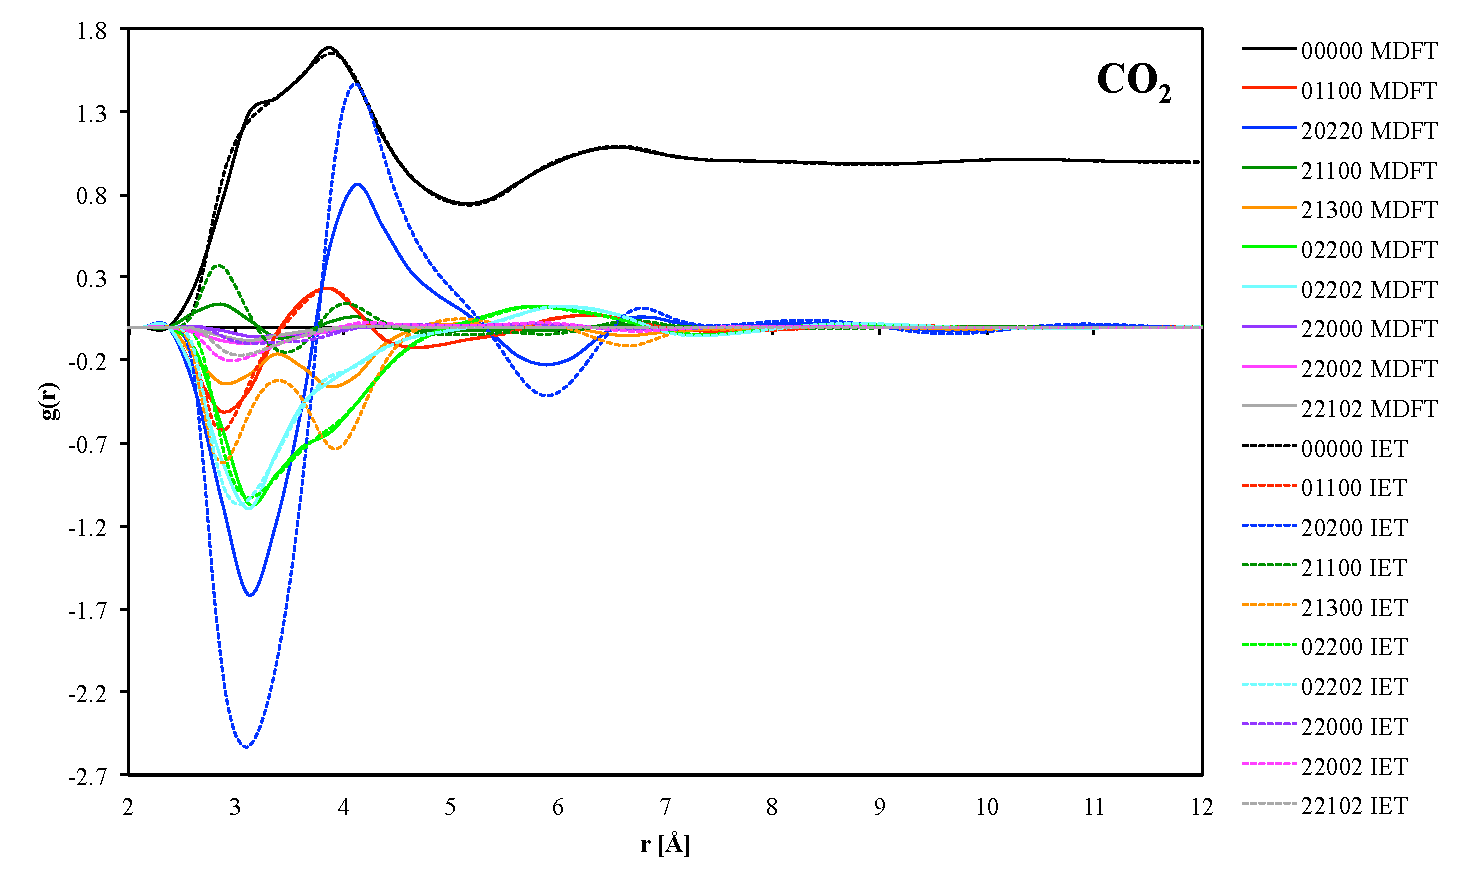
\includegraphics[width=1\columnwidth]{_figure/results/co2}
\par\end{centering}
\caption[The projections $\rho_{\mu\nu}^{mnl}(r)$ of $\mathrm{CO}_{2}$ comparing
to \acs{IET}]{The projections $\rho_{\mu\nu}^{mnl}(r)$ of $\mathrm{CO}_{2}$ comparing
to \acs{IET}, with $m_{\max}=n_{\max}=5$, $L=24$ $\textrm{Å}$,
$\mathrm{nfft}=72$. $\frac{1}{3}n_{\mathrm{bin}}$ is used in order
to avoid noise.\label{fig:Comparison-co2}}
\end{figure}


\section{First conclusion}

From the above results, the following first conclusions may be drawn:
\begin{itemize}
\item \acs{MDFT} is capable to produce the solvation free energy at chemical
precision with normal convergence criteria (which gives 2 decimal
for a specific spatial and angular grid), which is nearly the same
compared to mathematical equivalent \acs{IET} results for LJ centers,
single ions and linear solutes. The variance of free energy due to
discretization parameters is at chemical precision, i.e. 1 to 2 kJ/mol.
To keep this precision, at least $n_{\max}=3$ is needed, and the
order of quadrature $m_{\max}$ has no influence to the energy and
structure if it is larger than $n_{\max}$. This $n_{\max}$ is far
from sufficient to describe the solvent density $\rho$, but sufficient
for $\gamma$. As $\rho$ is produced by the minimization, its expansion
has no influence to the final result. The different branches produce
almost the same result with the same \acs{DCF}, comparing to the
error introduced by spatial grid dependence; while \texttt{\textbf{naive\_interpolation}}
seems to be a bit more stable compared to \texttt{\textbf{convolution}}
methods in terms of convergence for negative molecules, but exhibits
a small an energy shift about 2 kJ/mol for neutral LJ centers. For
charged solutes, the two types of free energy corrections mentioned
in this thesis are needed.
\item As for structure, \acs{MDFT} can also produce the same result as
\acs{IET}. It requires about $n_{\max}=4$ to have a converged curve
of $g(r)$ projections. For solutes, we are obliged to use looser
sampling rate to have a smooth curve; as the spatial grid is cubic,
but not in spherical coordinates as \acs{IET}. Indeed \acs{MDFT}
has the great advantage to be generalizable to produce 3D solvent
structures for complicate molecules, but \acs{IET} is ideal, and
much more efficient, to give information about small symmetric molecules
using functions with respect to $r$.
\end{itemize}

